\chapter{Interactive Workload}
\label{section:interactive}

This workload consists of a set of relatively complex read-only queries, that touch a significant
amount of data -- often the two-step friendship neighborhood and associated messages --, but typically in close proximity to a single node. Hence, the query complexity is sublinear to the dataset size.

The LDBC SNB Interactive workload consists of four query classes:

\begin{itemize}
\item \textbf{Complex read-only queries.} See \autoref{sec:complex-reads}.
\item \textbf{Short read-only queries.} See \autoref{sec:short-reads}.
\item \textbf{Transactional insert queries.} See \autoref{sec:inserts}.
\item \textbf{Transactional delete queries.} See \autoref{sec:deletes}.
\end{itemize}

A detailed description of the workload is available in the paper published at \mbox{SIGMOD} 2015~\cite{DBLP:conf/sigmod/ErlingALCGPPB15}.

%%%%%%%%%%%%%%%%%%%%%%%%%%%%%%%%%%%%%%%%%%%%%%%%%%%%%%%%%%%%%%%%%%%%%%%%%%%%%%
%%%%%%%%%%%%%%%%%%%%%%%%%%%%%%%%%%%%%%%%%%%%%%%%%%%%%%%%%%%%%%%%%%%%%%%%%%%%%%
%%%%%%%%%%%%%%%%%%%%%%%%%%%%%%%%%%%%%%%%%%%%%%%%%%%%%%%%%%%%%%%%%%%%%%%%%%%%%%

\section{Complex Reads}
\label{sec:complex-reads}

\renewcommand*{\arraystretch}{1.1}

\subsection*{Interactive / complex / 1}
\label{section:interactive-complex-read-01}

% change \emph{} to use sans-serif font
\let\oldemph\emph
\renewcommand{\emph}[1]{{\footnotesize \sf #1}}

\renewcommand{\currentQueryCard}{1}
\marginpar{
	\raggedleft
	\vspace{0.22ex}

	\queryRefCard{interactive-complex-read-01}{IC}{1}\\
	\queryRefCard{interactive-complex-read-02}{IC}{2}\\
	\queryRefCard{interactive-complex-read-03}{IC}{3}\\
	\queryRefCard{interactive-complex-read-04}{IC}{4}\\
	\queryRefCard{interactive-complex-read-05}{IC}{5}\\
	\queryRefCard{interactive-complex-read-06}{IC}{6}\\
	\queryRefCard{interactive-complex-read-07}{IC}{7}\\
	\queryRefCard{interactive-complex-read-08}{IC}{8}\\
	\queryRefCard{interactive-complex-read-09}{IC}{9}\\
	\queryRefCard{interactive-complex-read-10}{IC}{10}\\
	\queryRefCard{interactive-complex-read-11}{IC}{11}\\
	\queryRefCard{interactive-complex-read-12}{IC}{12}\\
	\queryRefCard{interactive-complex-read-13}{IC}{13}\\
	\queryRefCard{interactive-complex-read-14}{IC}{14}\\
}


\noindent\begin{tabularx}{\queryCardWidth}{|>{\queryPropertyCell}p{\queryPropertyCellWidth}|X|}
	\hline
	query & Interactive / complex / 1 \\ \hline
%
	title & Friends with certain name \\ \hline
%
	pattern & \multicolumn{1}{c|}{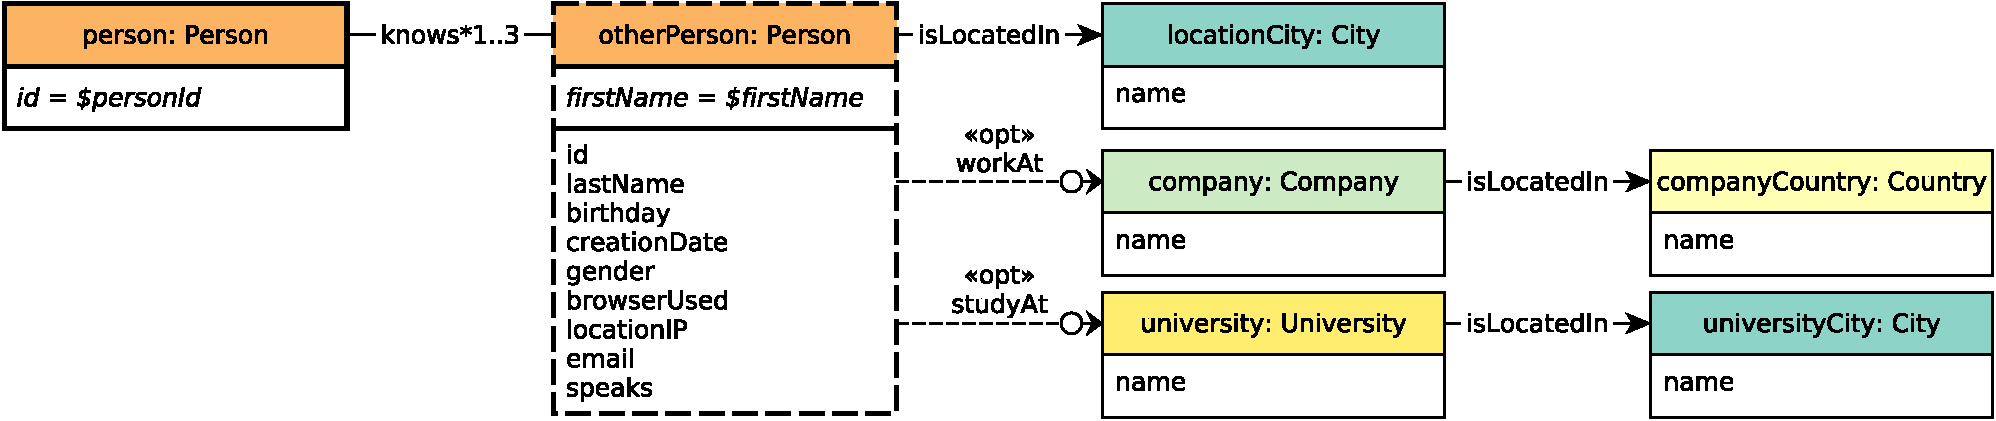
\includegraphics[scale=\patternscale,margin=0cm .2cm]{patterns/interactive-complex-read-01}} \\ \hline
%
	desc. & Given a start Person, find Persons with a given first name that the
start Person is connected to (excluding start Person) by at most 3 steps
via Knows relationships. Return Persons, including summaries of the
Persons workplaces and places of study.
 \\ \hline
%
	
		params &
		\innerCardVSpace{\begin{tabularx}{\attributeCardWidth}{|>{\paramNumberCell}c|>{\varNameCell}M|>{\typeCell}m{\typeWidth}|Y|} \hline
		$\mathsf{1}$ & Person.id
 & ID
 &  \\ \hline
		$\mathsf{2}$ & Person.firstName
 & String
 &  \\ \hline
		\end{tabularx}}\innerCardVSpace \\ \hline
	
%
	
		result &
		\innerCardVSpace{\begin{tabularx}{\attributeCardWidth}{|>{\resultNumberCell}c|>{\varNameCell}M|>{\typeCell}m{\typeWidth}|>{\resultOriginCell}c|Y|} \hline
		$\mathsf{1}$ & Person.id & ID & R &
				 \\ \hline
		$\mathsf{2}$ & Person.lastName & String & R &
				 \\ \hline
		$\mathsf{3}$ & distanceFromPerson & 32-bit Integer & R &
				1..3
 \\ \hline
		$\mathsf{4}$ & Person.birthday & Date & R &
				 \\ \hline
		$\mathsf{5}$ & Person.creationDate & DateTime & R &
				 \\ \hline
		$\mathsf{6}$ & Person.gender & String & R &
				 \\ \hline
		$\mathsf{7}$ & Person.browserUsed & String & R &
				 \\ \hline
		$\mathsf{8}$ & Person.locationIP & String & R &
				 \\ \hline
		$\mathsf{9}$ & \{Person.email\} & \{String\} & R &
				 \\ \hline
		$\mathsf{10}$ & \{Person.speaks\} & \{String\} & R &
				 \\ \hline
		$\mathsf{11}$ & Person-isLocatedIn-\textgreater{}Place.name & String & R &
				 \\ \hline
		$\mathsf{12}$ & \{Person-studyAt-\textgreater{}University.name,
Person-studyAt-\textgreater{}.classYear,
Person-studyAt-\textgreater{}University-isLocatedIn-\textgreater{}City.name\} & \{\textless{}String, 32-bit Integer, String\textgreater{}\} & R &
				 \\ \hline
		$\mathsf{13}$ & \{Person-workAt-\textgreater{}Company.name,
Person-workAt-\textgreater{}.workFrom,
Person-workAt-\textgreater{}Company-isLocatedIn-\textgreater{}Country.name\} & \{\textless{}String, 32-bit Integer, String\textgreater{}\} & R &
				 \\ \hline
		\end{tabularx}}\innerCardVSpace \\ \hline
	
%
	
		sort		&
		\innerCardVSpace{\begin{tabularx}{\attributeCardWidth}{|>{\sortNumberCell}c|>{\varNameCell}M|>{\directionCell}c|Y|} \hline
		$\mathsf{1}$ & distanceFromPerson
 & $\asc
$ &  \\ \hline
		$\mathsf{2}$ & Person.lastName
 & $\asc
$ &  \\ \hline
		$\mathsf{3}$ & Person.id
 & $\asc
$ &  \\ \hline
		\end{tabularx}}\innerCardVSpace \\ \hline
	%
	limit & 20 \\ \hline
	%
	CPs &
	\multicolumn{1}{>{\raggedright}l|}{
		\chokePoint{2.1}, 
		\chokePoint{5.3}
		} \\ \hline
	%
	relevance &
		\footnotesize This query is a representative of a simple navigational query. It looks for paths of length 1..3 through
the knows relation, starting from a given Person and ending at a Person with a given first name. It is interesting for several
aspects. (1) It requires for a complex aggregation for returning the concatenation of universities, companies,
languages and email information of the person. (2) It tests the ability of the optimizer to move the evaluation of
sub-queries functionally dependant on the Person, after the evaluation of the top-k. (3) Its performance is
highly sensitive to properly estimating the cardinalities in each transitive path, and paying attention not to explore
already visited Persons.
 \\ \hline%
\end{tabularx}
\queryCardVSpace

% change \emph back to the old one
\let\emph\oldemph
\renewcommand*{\arraystretch}{1.1}

\noindent\begin{tabularx}{17cm}{|>{\small \sf}c|X|}
	\hline
	query    & Interactive / complex / 2 \\ \hline
%
	title       & Recent posts and comments by your friends \\ \hline
%
    pattern     & \hfill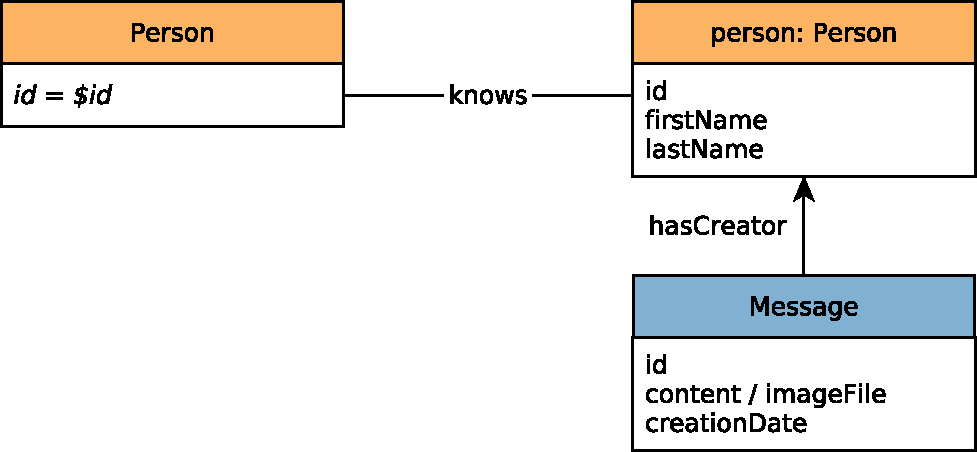
\includegraphics[scale=\patternscale,margin=0cm .2cm]{patterns/interactive-complex-read-02}\hfill\vadjust{} \\ \hline
%
	desc. & Given a start Person, find (most recent) Messages from all of that
Person's friends, that were created before (and including) a given date.
 \\ \hline
%
	
%
	params.  &
	\vspace{1.1ex}{\begin{tabularx}{14.2cm}{|c|M|m{2cm}|Y|} \hline
	\cellcolor{parameter} \color{white} $\mathsf{1}$ & \varname{Person.id} & \cellcolor{gray!20} \vartype{ID} &  \\ \hline
	\cellcolor{parameter} \color{white} $\mathsf{2}$ & \varname{date} & \cellcolor{gray!20} \vartype{DateTime} &  \\ \hline
	\end{tabularx}}\vspace{1.1ex} \\ \hline
%
	
	result      &
	\vspace{1.1ex}{\begin{tabularx}{14.2cm}{|c|M|m{2cm}|c|Y|} \hline
	\cellcolor{result} \color{white} $\mathsf{1}$ & \varname{Message-hasCreator->Person.id} & \cellcolor{gray!20} \vartype{ID} &
	    \texttt{R} &
	     \\ \hline
	\cellcolor{result} \color{white} $\mathsf{2}$ & \varname{Message-hasCreator->Person.firstName} & \cellcolor{gray!20} \vartype{String} &
	    \texttt{R} &
	     \\ \hline
	\cellcolor{result} \color{white} $\mathsf{3}$ & \varname{Message-hasCreator->Person.lastName} & \cellcolor{gray!20} \vartype{String} &
	    \texttt{R} &
	     \\ \hline
	\cellcolor{result} \color{white} $\mathsf{4}$ & \varname{Message.id} & \cellcolor{gray!20} \vartype{ID} &
	    \texttt{R} &
	     \\ \hline
	\cellcolor{result} \color{white} $\mathsf{5}$ & \varname{Message.content or Post.imageFile} & \cellcolor{gray!20} \vartype{String} &
	    \texttt{R} &
	     \\ \hline
	\cellcolor{result} \color{white} $\mathsf{6}$ & \varname{Message.creationDate} & \cellcolor{gray!20} \vartype{DateTime} &
	    \texttt{R} &
	     \\ \hline
	\end{tabularx}}\vspace{1.1ex} \\ \hline
	
%
	sort        &
	\vspace{1.1ex}{\begin{tabular}{|c|l|c|} \hline
	\cellcolor{sort} \color{white} $\mathsf{1}$ & \varname{Message.creationDate} & \cellcolor{gray!20} $\desc$ \\ \hline
	\cellcolor{sort} \color{white} $\mathsf{2}$ & \varname{Message.id} & \cellcolor{gray!20} $\asc$ \\ \hline
	\end{tabular}}\vspace{1.1ex} \\ \hline
	%
	limit       & 20 \\ \hline
	%
	CPs &
	\multicolumn{1}{>{\raggedright}l|}{
	  \chokepoint{1.1}, 
	  \chokepoint{2.2}, 
	  \chokepoint{2.3}, 
	  \chokepoint{3.2}
	  } \\ \hline
	%
    relevance &
      \small This is a navigational query looking for paths of length two, starting from a given Person, going to their friends and
from them, moving to their published Posts and Comments. This query exercices both the optimizer and how data is
stored. It tests the ability to create execution plans taking advantage of the orderings induced by some operators to
avoid performing expensive sorts. This query requires selecting Posts and Comments based on their creation date,
which might be correlated with their identifier and therefore, having intermediate results with interesting orders.
Also, messages could be stored in an order correlated with their creation date to improve data access locality. Finally,
as many of the attributes required in the projection are not needed for the execution of the query, it is expected that
the query optimizer will move the projection to the end.
 \\ \hline%
\end{tabularx}
\vspace{2ex}
\renewcommand*{\arraystretch}{1.1}

\noindent\begin{tabularx}{17cm}{|>{\small \sf}c|X|}
	\hline
	query    & Interactive / complex / 3 \\ \hline
%
	title       & Friends and friends of friends that have been to countries X and Y \\ \hline
%
    pattern     & \hfill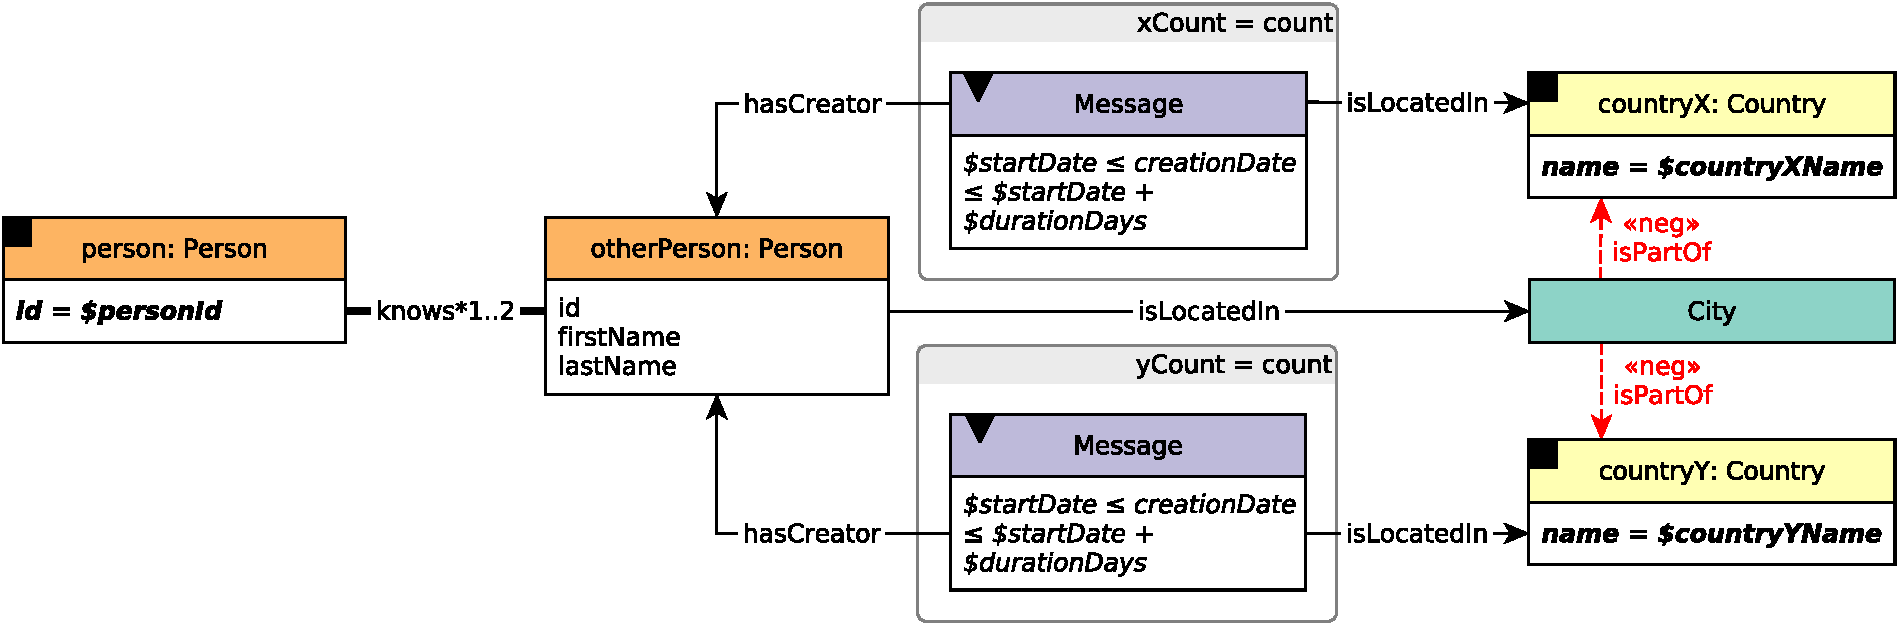
\includegraphics[scale=\patternscale,margin=0cm .2cm]{patterns/interactive-complex-read-03}\hfill\vadjust{} \\ \hline
%
	desc. & Given a start Person, find Persons that are their friends and friends of
friends (excluding start Person) that have made Posts/Comments in both
of the given Countries, X and Y, within a given period. Only Persons
that are foreign to Countries X and Y are considered, that is Persons
whose Location is not Country X or Country Y.
 \\ \hline
%
	
%
	params.  &
	\vspace{1.1ex}{\begin{tabularx}{14.66cm}{|c|M|m{2cm}|Y|} \hline
	\cellcolor{parameter} \color{white} $\mathsf{1}$ & \varname{Person.id} & \cellcolor{gray!20} \vartype{ID} &  \\ \hline
	\cellcolor{parameter} \color{white} $\mathsf{2}$ & \varname{CountryX.name} & \cellcolor{gray!20} \vartype{String} &  \\ \hline
	\cellcolor{parameter} \color{white} $\mathsf{3}$ & \varname{CountryY.name} & \cellcolor{gray!20} \vartype{String} &  \\ \hline
	\cellcolor{parameter} \color{white} $\mathsf{4}$ & \varname{startDate} & \cellcolor{gray!20} \vartype{Date} & beginning of requested period \\ \hline
	\cellcolor{parameter} \color{white} $\mathsf{5}$ & \varname{duration} & \cellcolor{gray!20} \vartype{32-bit Integer} & duration of requested period, in days the interval [startDate, startDate + Duration) is closed-open \\ \hline
	\end{tabularx}}\vspace{1.1ex} \\ \hline
%
	
	result      &
	\vspace{1.1ex}{\begin{tabularx}{14.66cm}{|c|M|m{2cm}|c|Y|} \hline
	\cellcolor{result} \color{white} $\mathsf{1}$ & \varname{Person.id} & \cellcolor{gray!20} \vartype{ID} &
	    \texttt{R} &
	     \\ \hline
	\cellcolor{result} \color{white} $\mathsf{2}$ & \varname{Person.firstName} & \cellcolor{gray!20} \vartype{String} &
	    \texttt{R} &
	     \\ \hline
	\cellcolor{result} \color{white} $\mathsf{3}$ & \varname{Person.lastName} & \cellcolor{gray!20} \vartype{String} &
	    \texttt{R} &
	     \\ \hline
	\cellcolor{result} \color{white} $\mathsf{4}$ & \varname{countX} & \cellcolor{gray!20} \vartype{32-bit Integer} &
	    \texttt{A} &
	    number of Messages from Country X made by Person within the given time \\ \hline
	\cellcolor{result} \color{white} $\mathsf{5}$ & \varname{countY} & \cellcolor{gray!20} \vartype{32-bit Integer} &
	    \texttt{A} &
	    number of Messages from Country Y made by Person within the given time \\ \hline
	\cellcolor{result} \color{white} $\mathsf{6}$ & \varname{count} & \cellcolor{gray!20} \vartype{32-bit Integer} &
	    \texttt{A} &
	    countX + countY \\ \hline
	\end{tabularx}}\vspace{1.1ex} \\ \hline
	
%
	sort        &
	\vspace{1.1ex}{\begin{tabular}{|c|l|c|} \hline
	\cellcolor{sort} \color{white} $\mathsf{1}$ & \varname{countX} & \cellcolor{gray!20} $\desc$ \\ \hline
	\cellcolor{sort} \color{white} $\mathsf{2}$ & \varname{Person.id} & \cellcolor{gray!20} $\asc$ \\ \hline
	\end{tabular}}\vspace{1.1ex} \\ \hline
	%
	limit       & 20 \\ \hline
	%
	CPs &
	\multicolumn{1}{>{\raggedright}l|}{
	  \chokepoint{2.1}, 
	  \chokepoint{3.1}, 
	  \chokepoint{5.1}
	  } \\ \hline
	%
    relevance &
      \small This query looks for paths of length two and three, starting from a Person, going to friends or friends of friends, and
then moving to Messages. This query tests the ability of the query optimizer to select the most efficient join ordering,
which will depend on the cardinalities of the intermediate results. Many friends of friends can be duplicate, then it is
expected to eliminate duplicates and those people prior to access the Post and Comments, as well as eliminate those
friends from countries X and Y, as the size of the intermediate results can be severely affected. A possible structural
optimization could be to materialize the number of Posts and Comments created by a person, and progressively
filter those people that could not even fall in the top 20 even having all their posts in the countries X and Y.
 \\ \hline%
\end{tabularx}
\vspace{2ex}
\renewcommand*{\arraystretch}{1.1}

\label{sec:interactive-complex-read-04}
\noindent\begin{tabularx}{\queryCardWidth}{|>{\queryPropertyCell}c|X|}
	\hline
	query & Interactive / complex / 4 \\ \hline
%
	title & New topics \\ \hline
%
    pattern & \hfill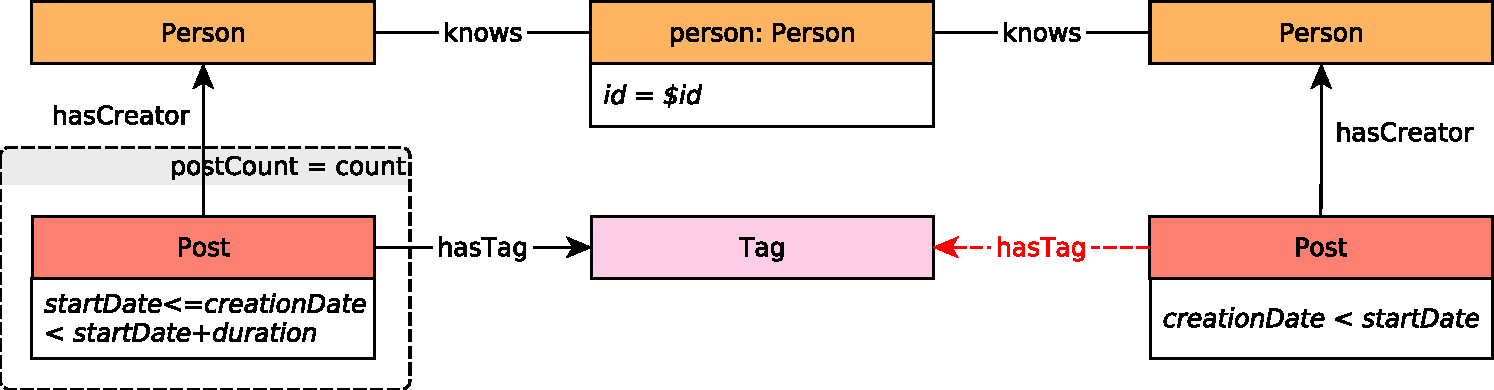
\includegraphics[scale=\patternscale,margin=0cm .2cm]{patterns/interactive-complex-read-04}\hfill\vadjust{} \\ \hline
%
	desc. & Given a start Person, find Tags that are attached to Posts that were
created by that Person's friends. Only include Tags that were attached
to friends' Posts created within a given time interval, and that were
never attached to friends' Posts created before this interval.
 \\ \hline
%
	
%
	params &
	\innerCardVSpace{\begin{tabularx}{\attributeCardWidth}{|>{\paramNumberCell}c|>{\varNameCell}M|>{\typeCell}m{\typeWidth}|Y|} \hline
	\cellcolor{parameter} \color{white} \footnotesize $\mathsf{1}$ &Person.id& ID &  \\ \hline
	\cellcolor{parameter} \color{white} \footnotesize $\mathsf{2}$ &startDate& Date &  \\ \hline
	\cellcolor{parameter} \color{white} \footnotesize $\mathsf{3}$ &duration& 32-bit Integer & duration of requested period, in days the interval [startDate, startDate + Duration) is closed-open \\ \hline
	\end{tabularx}}\innerCardVSpace \\ \hline
%
	
        result &
        \innerCardVSpace{\begin{tabularx}{\attributeCardWidth}{|>{\resultNumberCell}c|>{\varNameCell}M|>{\typeCell}m{\typeWidth}|>{\resultOriginCell}c|Y|} \hline
        $\mathsf{1}$ & Tag.name & String &R&
                 \\ \hline
        $\mathsf{2}$ & count & 32-bit Integer &A&
                number of Posts made within the given time interval that have this Tag \\ \hline
        \end{tabularx}}\innerCardVSpace \\ \hline
	
%
	sort        &
        \innerCardVSpace{\begin{tabular}{|>{\sortNumberCell}c|>{\varNameCell}l|>{\directionCell}c|} \hline
        $\mathsf{1}$ & count & $\desc$ \\ \hline
        $\mathsf{2}$ & Tag.name & $\asc$ \\ \hline
        \end{tabular}}\innerCardVSpace \\ \hline
	%
	limit & 10 \\ \hline
	%
	CPs &
	\multicolumn{1}{>{\raggedright}l|}{
	    \chokePoint{2.3}
	    } \\ \hline
	%
    relevance &
        \small This query looks for paths of length two, starting from a given Person, moving to Posts and then to Tags. It tests
the ability of the query optimizer to properly select the usage of hash joins or index based joins, depending on the
cardinality of the intermediate results. These cardinalities are clearly affected by the input Person, the number of
friends, the variety of Tags, the time interval and the number of Posts.
 \\ \hline%
\end{tabularx}
\queryCardVSpace
\renewcommand*{\arraystretch}{1.1}

\subsection*{Interactive / complex / 5}
\label{section:interactive-complex-read-05}

\noindent\begin{tabularx}{\queryCardWidth}{|>{\queryPropertyCell}p{\queryPropertyCellWidth}|X|}
	\hline
	query & Interactive / complex / 5 \\ \hline
%
	title & New groups
 \\ \hline
%
	pattern & \hfill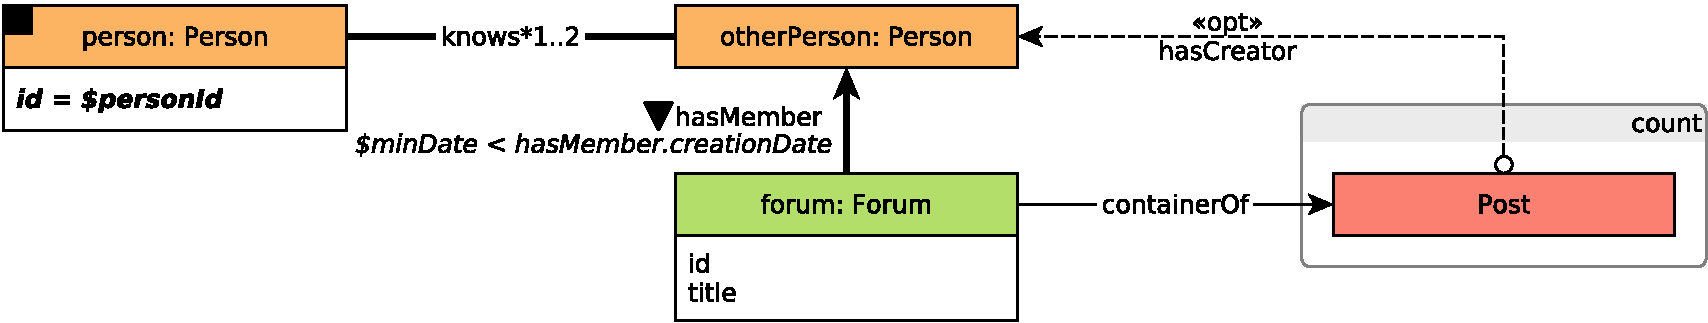
\includegraphics[scale=\patternscale,margin=0cm .2cm]{patterns/interactive-complex-read-05}\hfill\vadjust{} \\ \hline
%
	desc. & Given a start Person, find the Forums which that Person's friends and
friends of friends (excluding start Person) became Members of after a
given date. For each forum find the number of Posts that were created by
any of these Persons. For each Forum and consider only those Persons
which joined that particular Forum after the given date.
 \\ \hline
%
	
		params &
		\innerCardVSpace{\begin{tabularx}{\attributeCardWidth}{|>{\paramNumberCell}c|>{\varNameCell}M|>{\typeCell}m{\typeWidth}|Y|} \hline
		$\mathsf{1}$ & Person.id
 & ID
 &  \\ \hline
		$\mathsf{2}$ & date
 & Date
 &  \\ \hline
		\end{tabularx}}\innerCardVSpace \\ \hline
	
%
	
		result &
		\innerCardVSpace{\begin{tabularx}{\attributeCardWidth}{|>{\resultNumberCell}c|>{\varNameCell}M|>{\typeCell}m{\typeWidth}|>{\resultOriginCell}c|Y|} \hline
		$\mathsf{1}$ & Forum.title
 & String
 & R &
				 \\ \hline
		$\mathsf{2}$ & count
 & 32-bit Integer
 & R &
				Number of Posts made in Forum that were created by friends
 \\ \hline
		\end{tabularx}}\innerCardVSpace \\ \hline
	
%
	
		sort		&
		\innerCardVSpace{\begin{tabular}{|>{\sortNumberCell}c|>{\varNameCell}l|>{\directionCell}c|} \hline
		$\mathsf{1}$ & count
 & $\desc
$ \\ \hline
		$\mathsf{2}$ & Forum.id
 & $\asc
$ \\ \hline
		\end{tabular}}\innerCardVSpace \\ \hline
	%
	limit & 20 \\ \hline
	%
	CPs &
	\multicolumn{1}{>{\raggedright}l|}{
		\chokePoint{2.3}, 
		\chokePoint{3.3}
		} \\ \hline
	%
	relevance &
		\small This query looks for paths of length two and three, starting from a given Person, moving to friends and friends of
friends, and then getting the Forums they are members of. Besides testing the ability of the query optimizer to select
the proper join operator, it rewards the usage of indexes, but their accesses will be presumably scattered due to the
two/three-hop search space of the query, leading to unpredictable and scattered index accesses. Having efficient
implementations of such indexes will be highly beneficial.
 \\ \hline%
\end{tabularx}
\queryCardVSpace
\renewcommand*{\arraystretch}{1.1}

\subsection*{Interactive / complex / 6}
\label{section:interactive-complex-read-06}

% change \emph{} to use sans-serif font
\let\oldemph\emph
\renewcommand{\emph}[1]{{\footnotesize \sf #1}}

\renewcommand{\currentQueryCard}{6}
\marginpar{
	\raggedleft
	\vspace{0.22ex}

	\queryRefCard{interactive-complex-read-01}{IC}{1}\\
	\queryRefCard{interactive-complex-read-02}{IC}{2}\\
	\queryRefCard{interactive-complex-read-03}{IC}{3}\\
	\queryRefCard{interactive-complex-read-04}{IC}{4}\\
	\queryRefCard{interactive-complex-read-05}{IC}{5}\\
	\queryRefCard{interactive-complex-read-06}{IC}{6}\\
	\queryRefCard{interactive-complex-read-07}{IC}{7}\\
	\queryRefCard{interactive-complex-read-08}{IC}{8}\\
	\queryRefCard{interactive-complex-read-09}{IC}{9}\\
	\queryRefCard{interactive-complex-read-10}{IC}{10}\\
	\queryRefCard{interactive-complex-read-11}{IC}{11}\\
	\queryRefCard{interactive-complex-read-12}{IC}{12}\\
	\queryRefCard{interactive-complex-read-13}{IC}{13}\\
	\queryRefCard{interactive-complex-read-14}{IC}{14}\\
}


\noindent\begin{tabularx}{\queryCardWidth}{|>{\queryPropertyCell}p{\queryPropertyCellWidth}|X|}
	\hline
	query & Interactive / complex / 6 \\ \hline
%
	title & Tag co-occurrence \\ \hline
%
	pattern & \multicolumn{1}{c|}{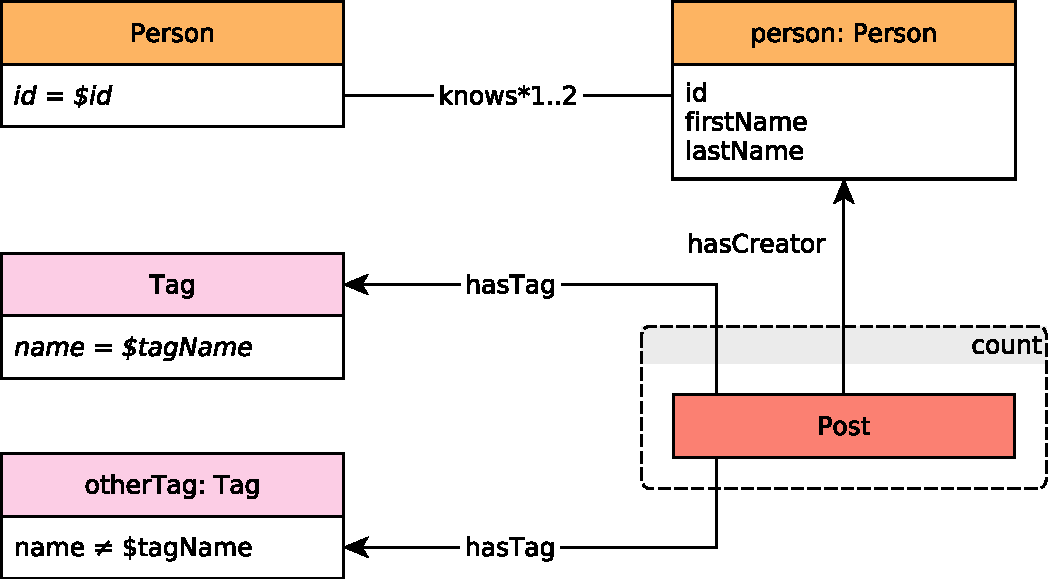
\includegraphics[scale=\patternscale,margin=0cm .2cm]{patterns/interactive-complex-read-06}} \\ \hline
%
	desc. & Given a start Person and some Tag, find the other Tags that occur
together with this Tag on Posts that were created by start Person's
friends and friends of friends (excluding start Person). Return For each
Tag, find the count of Posts that were created by these Persons, which
contain both this Tag and the given Tag.
 \\ \hline
%
	
		params &
		\innerCardVSpace{\begin{tabularx}{\attributeCardWidth}{|>{\paramNumberCell}c|>{\varNameCell}M|>{\typeCell}m{\typeWidth}|Y|} \hline
		$\mathsf{1}$ & Person.id
 & ID
 & \texttt{Person}
 \\ \hline
		$\mathsf{2}$ & Tag.name
 & String
 & \texttt{Tag}
 \\ \hline
		\end{tabularx}}\innerCardVSpace \\ \hline
	
%
	
		result &
		\innerCardVSpace{\begin{tabularx}{\attributeCardWidth}{|>{\resultNumberCell}c|>{\varNameCell}M|>{\typeCell}m{\typeWidth}|>{\resultOriginCell}c|Y|} \hline
		$\mathsf{1}$ & Tag.name & String & R &
				\texttt{tagName}
 \\ \hline
		$\mathsf{2}$ & postCount & 32-bit Integer & A &
				\texttt{postCount} -- Number of Posts that were created by friends and
friends of friends, which contain this Tag
 \\ \hline
		\end{tabularx}}\innerCardVSpace \\ \hline
	
%
	
		sort		&
		\innerCardVSpace{\begin{tabularx}{\attributeCardWidth}{|>{\sortNumberCell}c|>{\varNameCell}M|>{\directionCell}c|Y|} \hline
		$\mathsf{1}$ & postCount
 & $\desc
$ &  \\ \hline
		$\mathsf{2}$ & Tag.name
 & $\asc
$ &  \\ \hline
		\end{tabularx}}\innerCardVSpace \\ \hline
	%
	limit & 10 \\ \hline
	%
	CPs &
	\multicolumn{1}{>{\raggedright}l|}{
		\chokePoint{5.1}
		} \\ \hline
	%
	relevance &
		\footnotesize This query looks for paths of lengths three or four, starting from a Given Person, moving to friends or friends of
friends, then to Posts and finally ending at a given Tag.
 \\ \hline%
\end{tabularx}
\queryCardVSpace

% change \emph back to the old one
\let\emph\oldemph
\renewcommand*{\arraystretch}{1.1}

\subsection*{Interactive / complex / 7}
\label{section:interactive-complex-read-07}

% change \emph{} to use sans-serif font
\let\oldemph\emph
\renewcommand{\emph}[1]{{\footnotesize \sf #1}}

\renewcommand{\currentQueryCard}{7}
\marginpar{
	\raggedleft
	\vspace{0.22ex}

    \queryRefCard{interactive-complex-read-01}{IA}{1}\\
    \queryRefCard{interactive-complex-read-02}{IA}{2}\\
    \queryRefCard{interactive-complex-read-03}{IA}{3}\\
    \queryRefCard{interactive-complex-read-04}{IA}{4}\\
    \queryRefCard{interactive-complex-read-05}{IA}{5}\\
    \queryRefCard{interactive-complex-read-06}{IA}{6}\\
    \queryRefCard{interactive-complex-read-07}{IA}{7}\\
    \queryRefCard{interactive-complex-read-08}{IA}{8}\\
    \queryRefCard{interactive-complex-read-09}{IA}{9}\\
    \queryRefCard{interactive-complex-read-10}{IA}{10}\\
    \queryRefCard{interactive-complex-read-11}{IA}{11}\\
    \queryRefCard{interactive-complex-read-12}{IA}{12}\\
    \queryRefCard{interactive-complex-read-13}{IA}{13}\\
    \queryRefCard{interactive-complex-read-14}{IA}{14}\\
}


\noindent\begin{tabularx}{\queryCardWidth}{|>{\queryPropertyCell}p{\queryPropertyCellWidth}|X|}
	\hline
	query & Interactive / complex / 7 \\ \hline
%
	title & Recent likers
 \\ \hline
%
	pattern & \hfill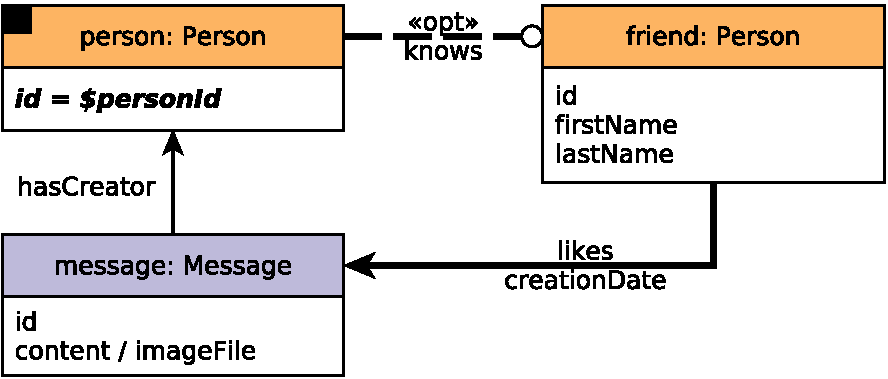
\includegraphics[scale=\patternscale,margin=0cm .2cm]{patterns/interactive-complex-read-07}\hfill\vadjust{} \\ \hline
%
	desc. & Given a start Person, find (most recent) Likes on any of start Person's
Messages. Find Persons that Liked any of start Person's Messages, the
Messages they liked most recently, creation date of that Like, and the
latency (in minutes) between creation of Messages and Like.
Additionally, for each Person found return a flag indicating whether the
liker is a friend of start Person. In the case that a Person Liked
multiple Messages at the same time, return the Message with lowest
identifier.
 \\ \hline
%
	
		params &
		\innerCardVSpace{\begin{tabularx}{\attributeCardWidth}{|>{\paramNumberCell}c|>{\varNameCell}M|>{\typeCell}m{\typeWidth}|Y|} \hline
		$\mathsf{1}$ & Person.id
 & 64-bit Integer
 &  \\ \hline
		\end{tabularx}}\innerCardVSpace \\ \hline
	
%
	
		result &
		\innerCardVSpace{\begin{tabularx}{\attributeCardWidth}{|>{\resultNumberCell}c|>{\varNameCell}M|>{\typeCell}m{\typeWidth}|>{\resultOriginCell}c|Y|} \hline
		$\mathsf{1}$ & Person.id & ID & R &
				 \\ \hline
		$\mathsf{2}$ & Person.firstName & String & R &
				 \\ \hline
		$\mathsf{3}$ & Person.lastName & String & R &
				 \\ \hline
		$\mathsf{4}$ & Like.creationDate & DateTime & R &
				 \\ \hline
		$\mathsf{5}$ & Message.id & ID & R &
				 \\ \hline
		$\mathsf{6}$ & Message.content or Post.imageFile & String & R &
				 \\ \hline
		$\mathsf{7}$ & latency & 32-bit Integer & C &
				Duration between creation of Message and Like, in minutes
 \\ \hline
		$\mathsf{8}$ & isNew & Boolean & C &
				\texttt{false} if liker Person is friend of start Person, \texttt{true}
otherwise
 \\ \hline
		\end{tabularx}}\innerCardVSpace \\ \hline
	
%
	
		sort		&
		\innerCardVSpace{\begin{tabularx}{\attributeCardWidth}{|>{\sortNumberCell}c|>{\varNameCell}M|>{\directionCell}c|Y|} \hline
		$\mathsf{1}$ & Like.creationDate
 & $\desc
$ &  \\ \hline
		$\mathsf{2}$ & Person.id
 & $\asc
$ &  \\ \hline
		\end{tabularx}}\innerCardVSpace \\ \hline
	%
	limit & 20 \\ \hline
	%
	CPs &
	\multicolumn{1}{>{\raggedright}l|}{
		\chokePoint{2.2}, 
		\chokePoint{2.3}, 
		\chokePoint{3.3}, 
		\chokePoint{5.1}
		} \\ \hline
	%
	relevance &
		\small This query looks for paths of length two, starting from a given Person, moving
to its published messages and then to Persons who liked them. It tests several aspects related to join optimization,
both at query optimization plan level and execution engine level. On the one hand, many of the columns needed for
the projection are only needed in the last stages of the query, so the optimizer is expected to delay the projection
until the end. This query implies accessing 2-hop data, and as a consequence, index accesses are expected to be
scattered. We expect to observe variate cardinalities, depending on the characteristics of the input parameter, so
properly selecting the join operators will be crucial. This query has a lot of correlated sub-queries, so it is testing
the ability to flatten the query execution plans.
 \\ \hline%
\end{tabularx}
\queryCardVSpace

% change \emph back to the old one
\renewcommand{\emph}[1]{\oldemph{#1}}
\renewcommand*{\arraystretch}{1.1}

\noindent\begin{tabularx}{17cm}{|p{1.95cm}|X|}
	\hline
	workload    & Interactive / complex \\ \hline
%
	query       & 8 \\ \hline
%
	title       & Recent replies \\ \hline
%
    pattern     & \hfill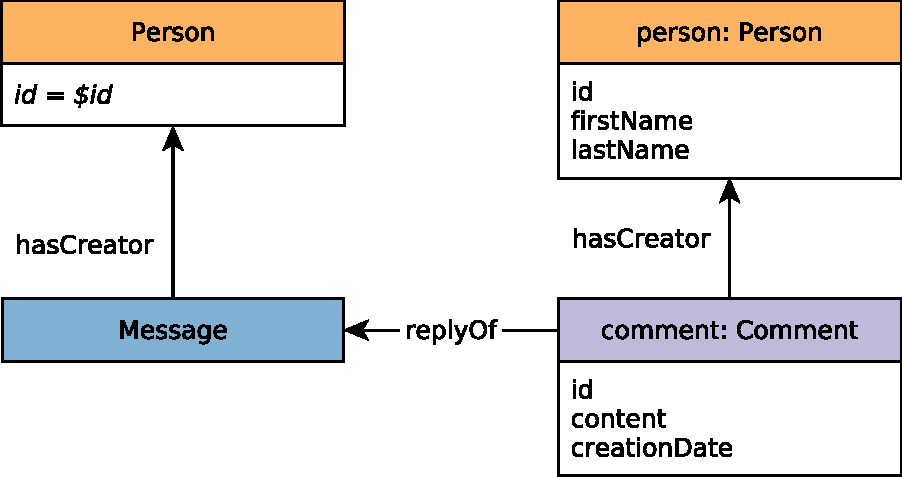
\includegraphics[scale=\patternscale,margin=0cm .2cm]{patterns/interactive-complex-read-08}\hfill\vadjust{} \\ \hline
%
	description & Given a start Person, find (most recent) Comments that are replies to
Messages of the start Person. Only consider immediate (1-hop) replies,
not the transitive (multi-hop) case. Return the reply Comments, and the
Person that created each reply Comment.
 \\ \hline
%
	
%
	parameters  &
	\vspace{1.1ex}{\begin{tabularx}{14.2cm}{|c|M|m{2cm}|Y|} \hline
	\cellcolor{parameter} \color{white} $\mathsf{1}$ & \varname{Person.id} & \cellcolor{gray!20} \vartype{ID} &  \\ \hline
	\end{tabularx}}\vspace{1.1ex} \\ \hline
%
	
	result      &
	\vspace{1.1ex}{\begin{tabularx}{14.2cm}{|c|M|m{2cm}|c|Y|} \hline
	\cellcolor{result} \color{white} $\mathsf{1}$ & \varname{Person.id} & \cellcolor{gray!20} \vartype{ID} &
	    \texttt{R} &
	     \\ \hline
	\cellcolor{result} \color{white} $\mathsf{2}$ & \varname{Person.firstName} & \cellcolor{gray!20} \vartype{String} &
	    \texttt{R} &
	     \\ \hline
	\cellcolor{result} \color{white} $\mathsf{3}$ & \varname{Person.lastName} & \cellcolor{gray!20} \vartype{String} &
	    \texttt{R} &
	     \\ \hline
	\cellcolor{result} \color{white} $\mathsf{4}$ & \varname{Comment.creationDate} & \cellcolor{gray!20} \vartype{DateTime} &
	    \texttt{R} &
	     \\ \hline
	\cellcolor{result} \color{white} $\mathsf{5}$ & \varname{Comment.id} & \cellcolor{gray!20} \vartype{ID} &
	    \texttt{R} &
	     \\ \hline
	\cellcolor{result} \color{white} $\mathsf{6}$ & \varname{Comment.content} & \cellcolor{gray!20} \vartype{String} &
	    \texttt{R} &
	     \\ \hline
	\end{tabularx}}\vspace{1.1ex} \\ \hline
	
%
	sort        &
	\vspace{1.1ex}{\begin{tabular}{|c|l|c|} \hline
	\cellcolor{sort} \color{white} $\mathsf{1}$ & \varname{Comment.creationDate} & \cellcolor{gray!20} $\desc$ \\ \hline
	\cellcolor{sort} \color{white} $\mathsf{2}$ & \varname{Comment.id} & \cellcolor{gray!20} $\asc$ \\ \hline
	\end{tabular}}\vspace{1.1ex} \\ \hline
	%
	limit       & 20 \\ \hline
	%
	%
\end{tabularx}
\vspace{2ex}
\renewcommand*{\arraystretch}{1.1}

\subsection*{Interactive / complex / 9}
\label{section:interactive-complex-read-09}

% change \emph{} to use sans-serif font
\let\oldemph\emph
\renewcommand{\emph}[1]{{\footnotesize \sf #1}}

\renewcommand{\currentQueryCard}{9}
\marginpar{
	\raggedleft
	\vspace{0.22ex}

	\queryRefCard{interactive-complex-read-01}{IC}{1}\\
	\queryRefCard{interactive-complex-read-02}{IC}{2}\\
	\queryRefCard{interactive-complex-read-03}{IC}{3}\\
	\queryRefCard{interactive-complex-read-04}{IC}{4}\\
	\queryRefCard{interactive-complex-read-05}{IC}{5}\\
	\queryRefCard{interactive-complex-read-06}{IC}{6}\\
	\queryRefCard{interactive-complex-read-07}{IC}{7}\\
	\queryRefCard{interactive-complex-read-08}{IC}{8}\\
	\queryRefCard{interactive-complex-read-09}{IC}{9}\\
	\queryRefCard{interactive-complex-read-10}{IC}{10}\\
	\queryRefCard{interactive-complex-read-11}{IC}{11}\\
	\queryRefCard{interactive-complex-read-12}{IC}{12}\\
	\queryRefCard{interactive-complex-read-13}{IC}{13}\\
	\queryRefCard{interactive-complex-read-14}{IC}{14}\\
}


\noindent\begin{tabularx}{\queryCardWidth}{|>{\queryPropertyCell}p{\queryPropertyCellWidth}|X|}
	\hline
	query & Interactive / complex / 9 \\ \hline
%
	title & Recent posts and comments by friends or friends of friends \\ \hline
%
	pattern & \multicolumn{1}{c|}{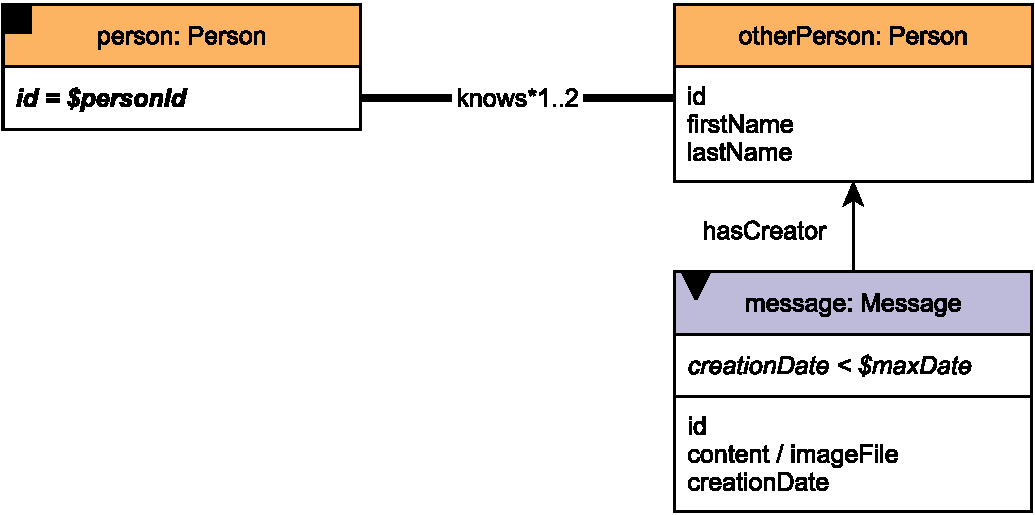
\includegraphics[scale=\patternscale,margin=0cm .2cm]{patterns/interactive-complex-read-09}} \\ \hline
%
	desc. & Given a start Person, find the (most recent) Messages created by that
Person's friends or friends of friends (excluding start Person). Only
consider the Messages created before a given date (excluding that date).
 \\ \hline
%
	
		params &
		\innerCardVSpace{\begin{tabularx}{\attributeCardWidth}{|>{\paramNumberCell}c|>{\varNameCell}M|>{\typeCell}m{\typeWidth}|Y|} \hline
		$\mathsf{1}$ & Person.id
 & ID
 &  \\ \hline
		$\mathsf{2}$ & date
 & Date
 &  \\ \hline
		\end{tabularx}}\innerCardVSpace \\ \hline
	
%
	
		result &
		\innerCardVSpace{\begin{tabularx}{\attributeCardWidth}{|>{\resultNumberCell}c|>{\varNameCell}M|>{\typeCell}m{\typeWidth}|>{\resultOriginCell}c|Y|} \hline
		$\mathsf{1}$ & Message-hasCreator-\textgreater{}Person.id & ID & R &
				\texttt{personId}
 \\ \hline
		$\mathsf{2}$ & Message-hasCreator-\textgreater{}Person.firstName & String & R &
				\texttt{personFirstName}
 \\ \hline
		$\mathsf{3}$ & Message-hasCreator-\textgreater{}Person.lastName & String & R &
				\texttt{personLastName}
 \\ \hline
		$\mathsf{4}$ & Message.id & ID & R &
				\texttt{commentOrPostId}
 \\ \hline
		$\mathsf{5}$ & Message.content or Post.imageFile & String & R &
				\texttt{commentOrPostContent}
 \\ \hline
		$\mathsf{6}$ & Message.creationDate & DateTime & R &
				\texttt{commentOrPostCreationDate}
 \\ \hline
		\end{tabularx}}\innerCardVSpace \\ \hline
	
%
	
		sort		&
		\innerCardVSpace{\begin{tabularx}{\attributeCardWidth}{|>{\sortNumberCell}c|>{\varNameCell}M|>{\directionCell}c|Y|} \hline
		$\mathsf{1}$ & Message.creationDate
 & $\desc
$ &  \\ \hline
		$\mathsf{2}$ & Message.id
 & $\asc
$ &  \\ \hline
		\end{tabularx}}\innerCardVSpace \\ \hline
	%
	limit & 20 \\ \hline
	%
	CPs &
	\multicolumn{1}{>{\raggedright}l|}{
		\chokePoint{1.1}, 
		\chokePoint{1.2}, 
		\chokePoint{2.2}, 
		\chokePoint{2.3}, 
		\chokePoint{3.2}, 
		\chokePoint{3.3}
		} \\ \hline
	%
	relevance &
		\footnotesize This query looks for paths of length two or three, starting from a given Person, moving to its friends and friends of
friends, and ending at their created Messages. This is one of the most complex queries, as the list of choke-points
indicates. This query is expected to touch variable amounts of data with entities of different characteristics, and
therefore, properly estimating cardinalities and selecting the proper operators will be crucial.
 \\ \hline%
\end{tabularx}
\queryCardVSpace

% change \emph back to the old one
\let\emph\oldemph
\renewcommand*{\arraystretch}{1.1}

\subsection*{Interactive / complex / 10}
\label{section:interactive-complex-read-10}

% change \emph{} to use sans-serif font
\let\oldemph\emph
\renewcommand{\emph}[1]{{\footnotesize \sf #1}}

\renewcommand{\currentQueryCard}{10}
\marginpar{
	\raggedleft
	\vspace{0.22ex}

	\queryRefCard{interactive-complex-read-01}{IC}{1}\\
	\queryRefCard{interactive-complex-read-02}{IC}{2}\\
	\queryRefCard{interactive-complex-read-03}{IC}{3}\\
	\queryRefCard{interactive-complex-read-04}{IC}{4}\\
	\queryRefCard{interactive-complex-read-05}{IC}{5}\\
	\queryRefCard{interactive-complex-read-06}{IC}{6}\\
	\queryRefCard{interactive-complex-read-07}{IC}{7}\\
	\queryRefCard{interactive-complex-read-08}{IC}{8}\\
	\queryRefCard{interactive-complex-read-09}{IC}{9}\\
	\queryRefCard{interactive-complex-read-10}{IC}{10}\\
	\queryRefCard{interactive-complex-read-11}{IC}{11}\\
	\queryRefCard{interactive-complex-read-12}{IC}{12}\\
	\queryRefCard{interactive-complex-read-13}{IC}{13}\\
	\queryRefCard{interactive-complex-read-14}{IC}{14}\\
}


\noindent\begin{tabularx}{\queryCardWidth}{|>{\queryPropertyCell}p{\queryPropertyCellWidth}|X|}
	\hline
	query & Interactive / complex / 10 \\ \hline
%
	title & Friend recommendation \\ \hline
%
	pattern & \multicolumn{1}{c|}{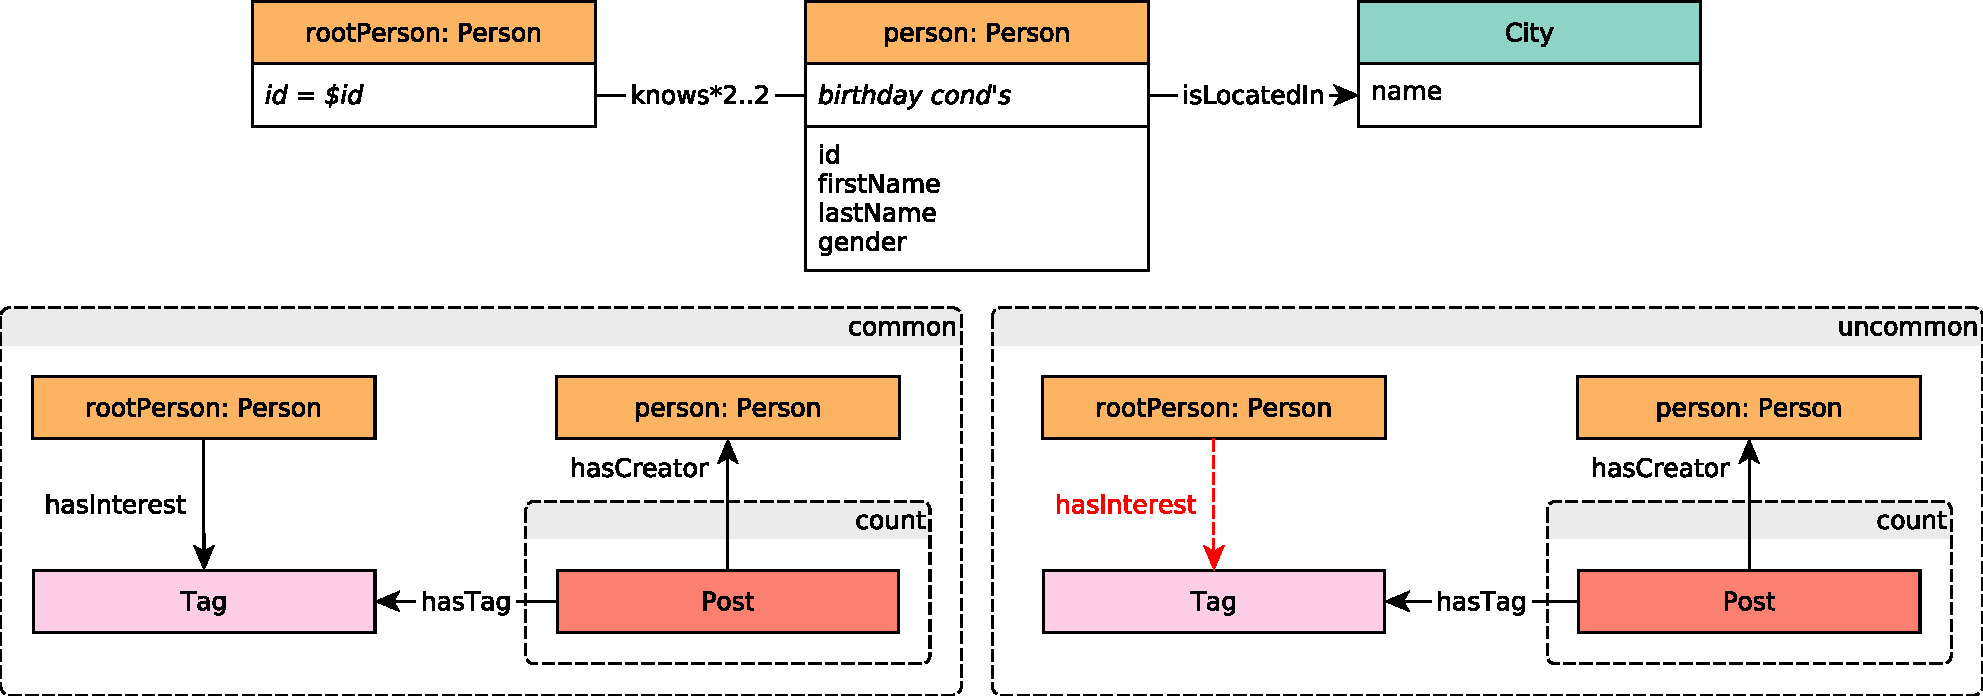
\includegraphics[scale=\patternscale,margin=0cm .2cm]{patterns/interactive-complex-read-10}} \\ \hline
%
	desc. & Given a start Person, find that Person's friends of friends (excluding
start Person, and immediate friends), who were born on or after the 21st
of a given month (in any year) and before the 22nd of the following
month. Calculate the similarity between each of these Persons and start
Person, where similarity for any Person is defined as follows:

\begin{itemize}
\tightlist
\item
  common = number of Posts created by that Person, such that the Post
  has a Tag that start Person is Interested in
\item
  uncommon = number of Posts created by that Person, such that the Post
  has no Tag that start Person is Interested in
\item
  similarity = common - uncommon
\end{itemize}
 \\ \hline
%
	
		params &
		\innerCardVSpace{\begin{tabularx}{\attributeCardWidth}{|>{\paramNumberCell}c|>{\varNameCell}M|>{\typeCell}m{\typeWidth}|Y|} \hline
		$\mathsf{1}$ & Person.id
 & ID
 &  \\ \hline
		$\mathsf{2}$ & month
 & 32-bit Integer
 & Between 1-12
 \\ \hline
		\end{tabularx}}\innerCardVSpace \\ \hline
	
%
	
		result &
		\innerCardVSpace{\begin{tabularx}{\attributeCardWidth}{|>{\resultNumberCell}c|>{\varNameCell}M|>{\typeCell}m{\typeWidth}|>{\resultOriginCell}c|Y|} \hline
		$\mathsf{1}$ & Person.id & ID & R &
				 \\ \hline
		$\mathsf{2}$ & Person.firstName & String & R &
				 \\ \hline
		$\mathsf{3}$ & Person.lastName & String & R &
				 \\ \hline
		$\mathsf{4}$ & similarity & 32-bit Integer & C &
				 \\ \hline
		$\mathsf{5}$ & Person.gender & String & R &
				 \\ \hline
		$\mathsf{6}$ & Person-isLocatedIn-\textgreater{}Place.name & String & R &
				 \\ \hline
		\end{tabularx}}\innerCardVSpace \\ \hline
	
%
	
		sort		&
		\innerCardVSpace{\begin{tabularx}{\attributeCardWidth}{|>{\sortNumberCell}c|>{\varNameCell}M|>{\directionCell}c|Y|} \hline
		$\mathsf{1}$ & similarity
 & $\desc
$ &  \\ \hline
		$\mathsf{2}$ & Person.id
 & $\asc
$ &  \\ \hline
		\end{tabularx}}\innerCardVSpace \\ \hline
	%
	limit & 10 \\ \hline
	%
	CPs &
	\multicolumn{1}{>{\raggedright}l|}{
		\chokePoint{2.3}, 
		\chokePoint{3.3}, 
		\chokePoint{4.1}, 
		\chokePoint{4.2}, 
		\chokePoint{5.1}, 
		\chokePoint{5.2}, 
		\chokePoint{6.1}, 
		\chokePoint{7.1}
		} \\ \hline
	%
	relevance &
		\footnotesize This query looks for paths of length two, starting from a Person and ending at the friends of their friends. It does
widely scattered graph traversal, and one expects no locality of in friends of friends, as these have been acquired
over a long time and have widely scattered identifiers. The join order is simple but one must see that the anti-join
for "not in my friends" is better with hash. Also the last pattern in the scalar sub-queries joining or anti-joining the
tags of the candidate's posts to interests of self should be by hash.
 \\ \hline%
\end{tabularx}
\queryCardVSpace

% change \emph back to the old one
\let\emph\oldemph
\renewcommand*{\arraystretch}{1.1}

\subsection*{Interactive / complex / 11}
\label{section:interactive-complex-read-11}

\noindent\begin{tabularx}{\queryCardWidth}{|>{\queryPropertyCell}p{\queryPropertyCellWidth}|X|}
	\hline
	query & Interactive / complex / 11 \\ \hline
%
	title & Job referral
 \\ \hline
%
	pattern & \hfill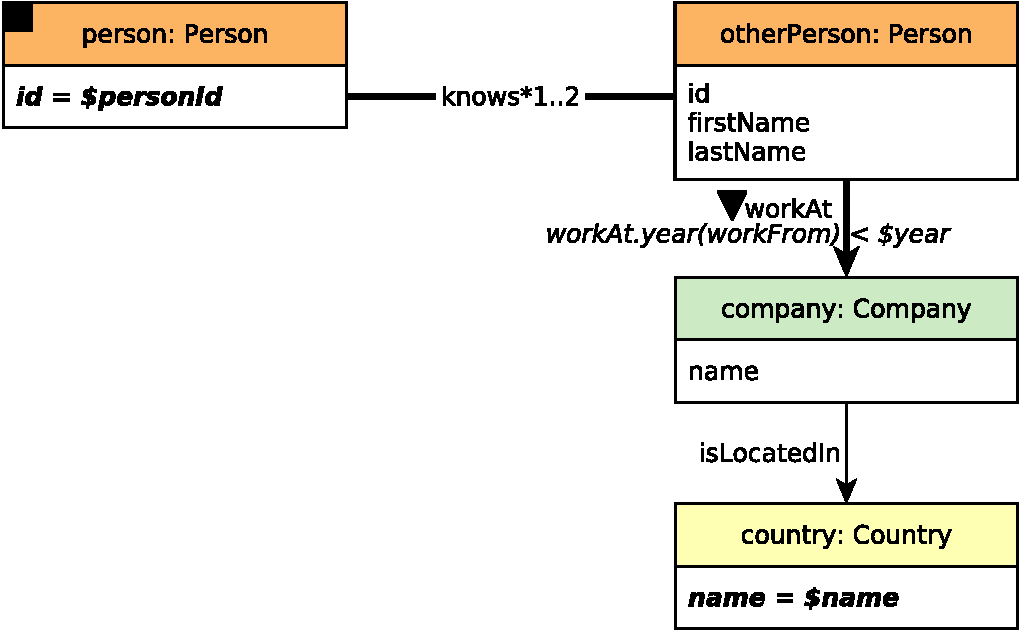
\includegraphics[scale=\patternscale,margin=0cm .2cm]{patterns/interactive-complex-read-11}\hfill\vadjust{} \\ \hline
%
	desc. & Given a start Person, find that Person's friends and friends of friends
(excluding start Person) who started Working in some Company in a given
Country, before a given date (year).
 \\ \hline
%
	
		params &
		\innerCardVSpace{\begin{tabularx}{\attributeCardWidth}{|>{\paramNumberCell}c|>{\varNameCell}M|>{\typeCell}m{\typeWidth}|Y|} \hline
		$\mathsf{1}$ & Person.id
 & ID
 &  \\ \hline
		$\mathsf{2}$ & Country.name
 & String
 &  \\ \hline
		$\mathsf{3}$ & year
 & 32-bit Integer
 &  \\ \hline
		\end{tabularx}}\innerCardVSpace \\ \hline
	
%
	
		result &
		\innerCardVSpace{\begin{tabularx}{\attributeCardWidth}{|>{\resultNumberCell}c|>{\varNameCell}M|>{\typeCell}m{\typeWidth}|>{\resultOriginCell}c|Y|} \hline
		$\mathsf{1}$ & Person.id
 & ID
 & R &
				 \\ \hline
		$\mathsf{2}$ & Person.firstName
 & String
 & R &
				 \\ \hline
		$\mathsf{3}$ & Person.lastName
 & String
 & R &
				 \\ \hline
		$\mathsf{4}$ & Person-worksAt-\textgreater{}Organisation.name
 & String
 & R &
				 \\ \hline
		$\mathsf{5}$ & Person-worksAt-\textgreater{}.worksFrom
 & 32-bit Integer
 & R &
				 \\ \hline
		\end{tabularx}}\innerCardVSpace \\ \hline
	
%
	
		sort		&
		\innerCardVSpace{\begin{tabularx}{\attributeCardWidth}{|>{\sortNumberCell}c|>{\varNameCell}M|>{\directionCell}c|Y|} \hline
		$\mathsf{1}$ & Person-worksAt-\textgreater{}.worksFrom
 & $\asc
$ &  \\ \hline
		$\mathsf{2}$ & Person.id
 & $\asc
$ &  \\ \hline
		$\mathsf{3}$ & Person-worksAt-\textgreater{}Organisation.name
 & $\desc
$ &  \\ \hline
		\end{tabularx}}\innerCardVSpace \\ \hline
	%
	limit & 10 \\ \hline
	%
	CPs &
	\multicolumn{1}{>{\raggedright}l|}{
		\chokePoint{1.4}, 
		\chokePoint{2.3}, 
		\chokePoint{2.4}, 
		\chokePoint{3.3}
		} \\ \hline
	%
	relevance &
		\small This query looks for paths of length two or three, starting from a Person, moving to friends or friends of friends,
and ending at a Company. In this query, there are selective joins and a top k order by that can be exploited for
optimizations.
 \\ \hline%
\end{tabularx}
\queryCardVSpace
\renewcommand*{\arraystretch}{1.1}

\subsection*{Interactive / complex / 12}
\label{section:interactive-complex-read-12}

% change \emph{} to use sans-serif font
\let\oldemph\emph
\renewcommand{\emph}[1]{{\footnotesize \sf #1}}

\renewcommand{\currentQueryCard}{12}
\marginpar{
	\raggedleft
	\vspace{0.22ex}

	\queryRefCard{interactive-complex-read-01}{IC}{1}\\
	\queryRefCard{interactive-complex-read-02}{IC}{2}\\
	\queryRefCard{interactive-complex-read-03}{IC}{3}\\
	\queryRefCard{interactive-complex-read-04}{IC}{4}\\
	\queryRefCard{interactive-complex-read-05}{IC}{5}\\
	\queryRefCard{interactive-complex-read-06}{IC}{6}\\
	\queryRefCard{interactive-complex-read-07}{IC}{7}\\
	\queryRefCard{interactive-complex-read-08}{IC}{8}\\
	\queryRefCard{interactive-complex-read-09}{IC}{9}\\
	\queryRefCard{interactive-complex-read-10}{IC}{10}\\
	\queryRefCard{interactive-complex-read-11}{IC}{11}\\
	\queryRefCard{interactive-complex-read-12}{IC}{12}\\
	\queryRefCard{interactive-complex-read-13}{IC}{13}\\
	\queryRefCard{interactive-complex-read-14}{IC}{14}\\
}


\noindent\begin{tabularx}{\queryCardWidth}{|>{\queryPropertyCell}p{\queryPropertyCellWidth}|X|}
	\hline
	query & Interactive / complex / 12 \\ \hline
%
	title & Expert search \\ \hline
%
	pattern & \centering 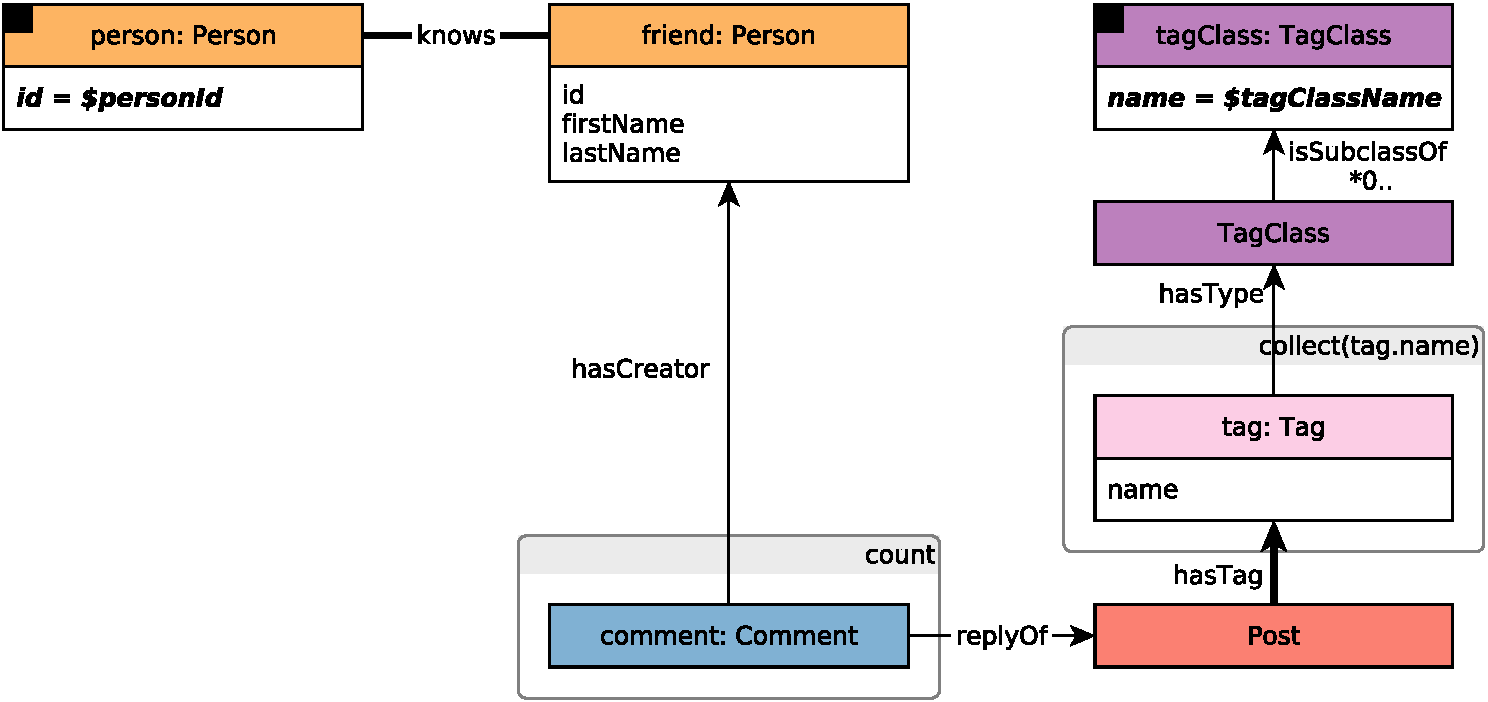
\includegraphics[scale=\patternscale,margin=0cm .2cm]{patterns/interactive-complex-read-12} \tabularnewline \hline
%
	desc. & Given a start Person, find the Comments that this Person's friends made
in reply to Posts, considering only those Comments that are immediate
(1-hop) replies to Posts, not the transitive (multi-hop) case. Only
consider Posts with a Tag in a given TagClass or in a descendent of that
TagClass. Count the number of these reply Comments, and collect the Tags
that were attached to the Posts they replied to, but only collect Tags
with the given TagClass or with a descendant of that TagClass Return
Persons with at least one reply, the reply count, and the collection of
Tags.
 \\ \hline
%
	
		params &
		\innerCardVSpace{\begin{tabularx}{\attributeCardWidth}{|>{\paramNumberCell}c|>{\varNameCell}M|>{\typeCell}m{\typeWidth}|Y|} \hline
		$\mathsf{1}$ & Person.id
 & ID
 & \texttt{personId}
 \\ \hline
		$\mathsf{2}$ & TagClass.name
 & String
 & \texttt{tagClassName}
 \\ \hline
		\end{tabularx}}\innerCardVSpace \\ \hline
	
%
	
		result &
		\innerCardVSpace{\begin{tabularx}{\attributeCardWidth}{|>{\resultNumberCell}c|>{\varNameCell}M|>{\typeCell}m{\typeWidth}|>{\resultOriginCell}c|Y|} \hline
		$\mathsf{1}$ & Person.id & ID & R &
				\texttt{personId}
 \\ \hline
		$\mathsf{2}$ & Person.firstName & String & R &
				\texttt{personFirstName}
 \\ \hline
		$\mathsf{3}$ & Person.lastName & String & R &
				\texttt{personLastName}
 \\ \hline
		$\mathsf{4}$ & \{Tag.name\} & \{String\} & R &
				\texttt{tagNames}
 \\ \hline
		$\mathsf{5}$ & replyCount & 32-bit Integer & A &
				\texttt{replyCount} -- Number of reply Comments
 \\ \hline
		\end{tabularx}}\innerCardVSpace \\ \hline
	
%
	
		sort		&
		\innerCardVSpace{\begin{tabularx}{\attributeCardWidth}{|>{\sortNumberCell}c|>{\varNameCell}M|>{\directionCell}c|Y|} \hline
		$\mathsf{1}$ & count
 & $\desc
$ &  \\ \hline
		$\mathsf{2}$ & Person.id
 & $\asc
$ &  \\ \hline
		\end{tabularx}}\innerCardVSpace \\ \hline
	%
	limit & 20 \\ \hline
	%
	CPs &
	\multicolumn{1}{>{\raggedright}l|}{
		\chokePoint{3.3}, 
		\chokePoint{7.2}, 
		\chokePoint{7.3}, 
		\chokePoint{8.2}
		} \\ \hline
	%
	relevance &
		\footnotesize This query looks for paths of length three, starting at a Person, moving to its friends, the to their Comments and
ending at the Post the Comments are replying. The chain from original post to the reply is transitive. The traversal
may be initiated at either end, the system may note that this is a tree, hence leaf to root is always best. Additionally,
a hash table can be built from either end, e.g. from the friends of self, from the tags in the category, from the or
other.
 \\ \hline%
\end{tabularx}
\queryCardVSpace

% change \emph back to the old one
\let\emph\oldemph
\renewcommand*{\arraystretch}{1.1}

\subsection*{Interactive / complex / 13}
\label{section:interactive-complex-read-13}

% change \emph{} to use sans-serif font
\let\oldemph\emph
\renewcommand{\emph}[1]{{\footnotesize \sf #1}}

\renewcommand{\currentQueryCard}{13}
\marginpar{
	\raggedleft
	\vspace{0.22ex}

	\queryRefCard{interactive-complex-read-01}{IC}{1}\\
	\queryRefCard{interactive-complex-read-02}{IC}{2}\\
	\queryRefCard{interactive-complex-read-03}{IC}{3}\\
	\queryRefCard{interactive-complex-read-04}{IC}{4}\\
	\queryRefCard{interactive-complex-read-05}{IC}{5}\\
	\queryRefCard{interactive-complex-read-06}{IC}{6}\\
	\queryRefCard{interactive-complex-read-07}{IC}{7}\\
	\queryRefCard{interactive-complex-read-08}{IC}{8}\\
	\queryRefCard{interactive-complex-read-09}{IC}{9}\\
	\queryRefCard{interactive-complex-read-10}{IC}{10}\\
	\queryRefCard{interactive-complex-read-11}{IC}{11}\\
	\queryRefCard{interactive-complex-read-12}{IC}{12}\\
	\queryRefCard{interactive-complex-read-13}{IC}{13}\\
	\queryRefCard{interactive-complex-read-14}{IC}{14}\\
}


\noindent\begin{tabularx}{\queryCardWidth}{|>{\queryPropertyCell}p{\queryPropertyCellWidth}|X|}
	\hline
	query & Interactive / complex / 13 \\ \hline
%
	title & Single shortest path \\ \hline
%
	pattern & \multicolumn{1}{c|}{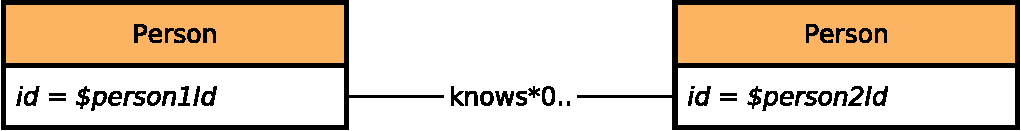
\includegraphics[scale=\patternscale,margin=0cm .2cm]{patterns/interactive-complex-read-13}} \\ \hline
%
	desc. & Given two Persons, find the shortest path between these two Persons in
the subgraph induced by the Knows relationships.

Return the length of this path:

\begin{itemize}
\tightlist
\item
  \(-1\) : no path found
\item
  \(0\): start person = end person
\item
  \(> 0\): regular case
\end{itemize}
 \\ \hline
%
	
		params &
		\innerCardVSpace{\begin{tabularx}{\attributeCardWidth}{|>{\paramNumberCell}c|>{\varNameCell}M|>{\typeCell}m{\typeWidth}|Y|} \hline
		$\mathsf{1}$ & person1.id
 & ID
 &  \\ \hline
		$\mathsf{2}$ & person2.id
 & ID
 &  \\ \hline
		\end{tabularx}}\innerCardVSpace \\ \hline
	
%
	
		result &
		\innerCardVSpace{\begin{tabularx}{\attributeCardWidth}{|>{\resultNumberCell}c|>{\varNameCell}M|>{\typeCell}m{\typeWidth}|>{\resultOriginCell}c|Y|} \hline
		$\mathsf{1}$ & length & 32-bit Integer & C &
				 \\ \hline
		\end{tabularx}}\innerCardVSpace \\ \hline
	
%
	%
	%
	CPs &
	\multicolumn{1}{>{\raggedright}l|}{
		\chokePoint{3.3}, 
		\chokePoint{7.2}, 
		\chokePoint{7.3}
		} \\ \hline
	%
	relevance &
		\small This query looks for a variable length path, starting at a given Person and finishing at an another given Person.
Proper cardinality estimation and search space prunning, will be crucial. This query also allows for possible parallel
implementations.
 \\ \hline%
\end{tabularx}
\queryCardVSpace

% change \emph back to the old one
\renewcommand{\emph}[1]{\oldemph{#1}}
\renewcommand*{\arraystretch}{1.1}

\noindent\begin{tabularx}{17cm}{|p{1.95cm}|X|}
	\hline
	workload    & Interactive / complex \\ \hline
%
	query       & 14 \\ \hline
%
	title       & Weighted/unweighted paths \\ \hline
%
    pattern     & \hfill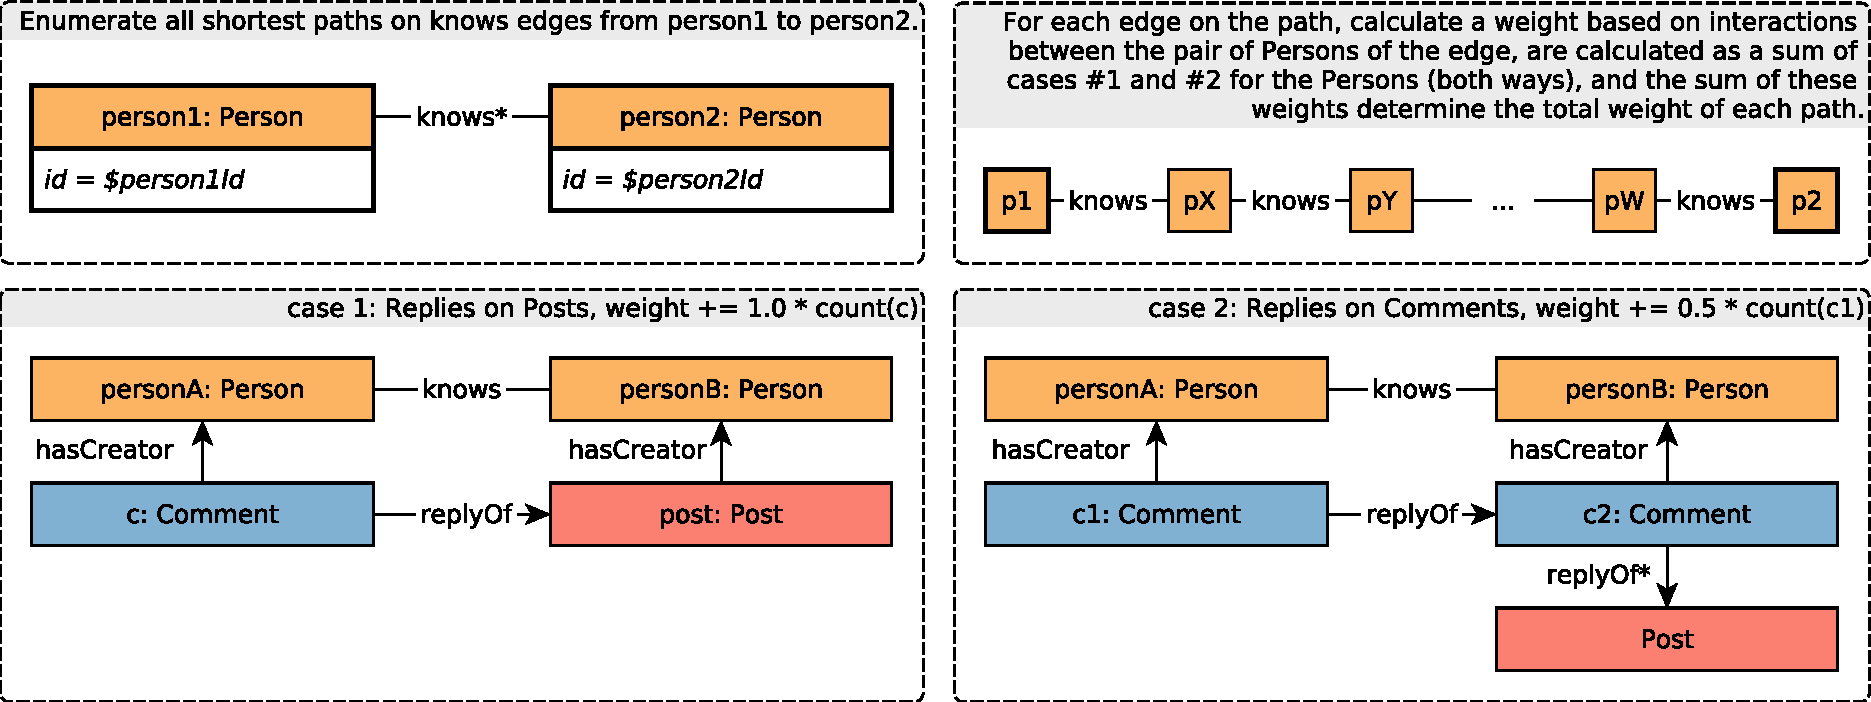
\includegraphics[scale=\patternscale,margin=0cm .2cm]{patterns/interactive-complex-read-14}\hfill\vadjust{} \\ \hline
%
	description & Given two Persons, find all (unweighted) shortest paths between these
two Persons, in the subgraph induced by the Knows relationship. Then,
for each path calculate a weight. The nodes in the path are Persons, and
the weight of a path is the sum of weights between every pair of
consecutive Person nodes in the path. The weight for a pair of Persons
is calculated such that every reply (by one of the Persons) to a Post
(by the other Person) contributes 1.0, and every reply (by ones of the
Persons) to a Comment (by the other Person) contributes 0.5. Return all
the paths with shortest length, and their weights.
 \\ \hline
%
	
%
	parameters  &
	\vspace{1.1ex}{\begin{tabularx}{14.2cm}{|c|M|m{2cm}|Y|} \hline
	\cellcolor{black!70} \color{white} $\mathsf{1}$ & \varname{person1.id} & \cellcolor{gray!20} \vartype{ID} &  \\ \hline
	\cellcolor{black!70} \color{white} $\mathsf{2}$ & \varname{person2.id} & \cellcolor{gray!20} \vartype{ID} &  \\ \hline
	\end{tabularx}}\vspace{1.1ex} \\ \hline
%
	
	result      &
	\vspace{1.1ex}{\begin{tabularx}{14.2cm}{|c|M|m{2cm}|Y|} \hline
	\cellcolor{black!70} \color{white} $\mathsf{1}$ & \varname{[Person.id]} & \cellcolor{gray!20} \vartype{[ID]} & Identifiers representing an ordered sequence of the Persons in the path \\ \hline
	\cellcolor{black!70} \color{white} $\mathsf{2}$ & \varname{weight} & \cellcolor{gray!20} \vartype{64-bit Float} &  \\ \hline
	\end{tabularx}}\vspace{1.1ex} \\ \hline
	
%
	sort        &
	\vspace{1.1ex}{\begin{tabular}{|c|l|c|} \hline
	\cellcolor{black!70} \color{white} $\mathsf{1}$ & \varname{weight} & \cellcolor{gray!20} $\desc$ \\ \hline
	\end{tabular}}\vspace{1.1ex} \\ \hline
	%
	%
	%
\end{tabularx}

%%%%%%%%%%%%%%%%%%%%%%%%%%%%%%%%%%%%%%%%%%%%%%%%%%%%%%%%%%%%%%%%%%%%%%%%%%%%%%
%%%%%%%%%%%%%%%%%%%%%%%%%%%%%%%%%%%%%%%%%%%%%%%%%%%%%%%%%%%%%%%%%%%%%%%%%%%%%%
%%%%%%%%%%%%%%%%%%%%%%%%%%%%%%%%%%%%%%%%%%%%%%%%%%%%%%%%%%%%%%%%%%%%%%%%%%%%%%

\section{Short Reads}
\label{sec:short-reads}

\renewcommand*{\arraystretch}{1.1}

\label{sec:interactive-short-read-01}
\noindent\begin{tabularx}{\queryCardWidth}{|>{\queryPropertyCell}c|X|}
	\hline
	query & Interactive / short / 1 \\ \hline
%
	title & Person Profile \\ \hline
%
    pattern & \hfill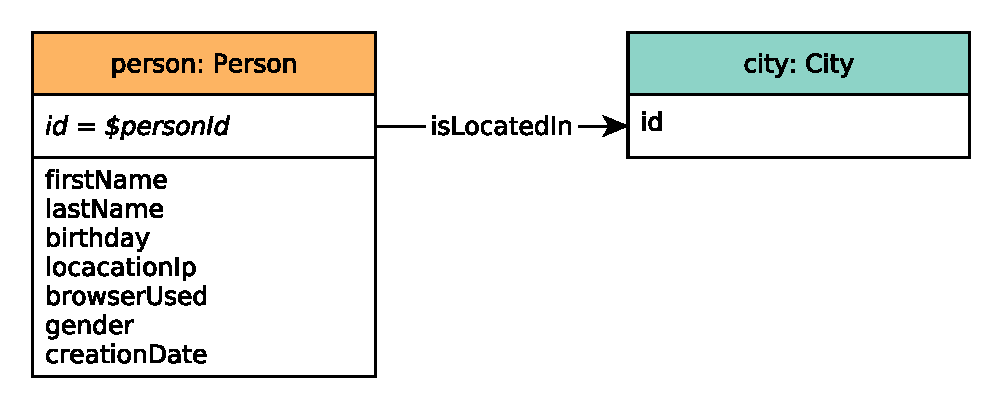
\includegraphics[scale=\patternscale,margin=0cm .2cm]{patterns/interactive-short-read-01}\hfill\vadjust{} \\ \hline
%
	desc. & Given a start Person, retrieve their first name, last name, birthday, IP
address, browser, and city of residence.
 \\ \hline
%
	
%
    
        params &
        \innerCardVSpace{\begin{tabularx}{\attributeCardWidth}{|>{\paramNumberCell}c|>{\varNameCell}M|>{\typeCell}m{\typeWidth}|Y|} \hline
        \cellcolor{parameter} \color{white} \footnotesize $\mathsf{1}$ &Person.id& ID &  \\ \hline
        \end{tabularx}}\innerCardVSpace \\ \hline
	
%
	
        result &
        \innerCardVSpace{\begin{tabularx}{\attributeCardWidth}{|>{\resultNumberCell}c|>{\varNameCell}M|>{\typeCell}m{\typeWidth}|>{\resultOriginCell}c|Y|} \hline
        $\mathsf{1}$ & Person.firstName & String &R&
                 \\ \hline
        $\mathsf{2}$ & Person.lastName & String &R&
                 \\ \hline
        $\mathsf{3}$ & Person.birthDay & Date &R&
                 \\ \hline
        $\mathsf{4}$ & Person.locationIP & String &R&
                 \\ \hline
        $\mathsf{5}$ & Person.browserUsed & String &R&
                 \\ \hline
        $\mathsf{6}$ & Person-isLocatedIn->Place.id & 32-bit Integer &R&
                 \\ \hline
        $\mathsf{7}$ & Person.gender & String &R&
                 \\ \hline
        $\mathsf{8}$ & Person.creationDate & DateTime &R&
                 \\ \hline
        \end{tabularx}}\innerCardVSpace \\ \hline
	
%
	%
	%
	%
    %
\end{tabularx}
\queryCardVSpace
\renewcommand*{\arraystretch}{1.1}

\noindent\begin{tabularx}{17cm}{|p{1.95cm}|X|}
	\hline
	workload    & Interactive / short \\ \hline
%
	query       & 2 \\ \hline
%
	title       & Person Recent Messages \\ \hline
%
    pattern     & \hfill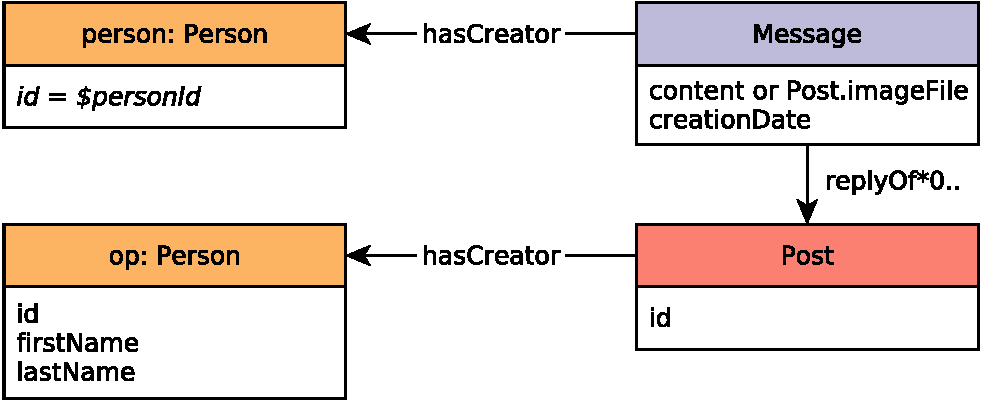
\includegraphics[scale=\patternscale,margin=0cm .2cm]{patterns/interactive-short-read-02}\hfill\vadjust{} \\ \hline
%
	description & Given a start Person, retrieve the last 10 Messages created by that
user. For each message, return that message, the original post in its
conversation, and the author of that post. If any of the Messages is a
Post, then the original Post will be the same Message, i.e.~that Message
will appear twice in that result.
 \\ \hline
%
	
%
	parameters  &
	\vspace{1.1ex}{\begin{tabularx}{14.2cm}{|c|M|m{2cm}|Y|} \hline
	\cellcolor{black!70} \color{white} $\mathsf{1}$ & \varname{Person.id} & \cellcolor{gray!20} \vartype{ID} &  \\ \hline
	\end{tabularx}}\vspace{1.1ex} \\ \hline
%
	
	result      &
	\vspace{1.1ex}{\begin{tabularx}{14.2cm}{|c|M|m{2cm}|Y|} \hline
	\cellcolor{black!70} \color{white} $\mathsf{1}$ & \varname{Message.id} & \cellcolor{gray!20} \vartype{64-bit Integer} &  \\ \hline
	\cellcolor{black!70} \color{white} $\mathsf{2}$ & \varname{Message.content or Post.imageFile} & \cellcolor{gray!20} \vartype{String} &  \\ \hline
	\cellcolor{black!70} \color{white} $\mathsf{3}$ & \varname{Message.creationDate} & \cellcolor{gray!20} \vartype{DateTime} &  \\ \hline
	\cellcolor{black!70} \color{white} $\mathsf{4}$ & \varname{Post.id or Comment-replyOf*->Post.id} & \cellcolor{gray!20} \vartype{ID} &  \\ \hline
	\cellcolor{black!70} \color{white} $\mathsf{5}$ & \varname{Post-hasCreator->Person.id or Comment-replyOf*->Post-hasCreator->Person.id} & \cellcolor{gray!20} \vartype{ID} &  \\ \hline
	\cellcolor{black!70} \color{white} $\mathsf{6}$ & \varname{Post-hasCreator->Person.firstName or Comment-replyOf*->Post-hasCreator->Person.firstName} & \cellcolor{gray!20} \vartype{String} &  \\ \hline
	\cellcolor{black!70} \color{white} $\mathsf{7}$ & \varname{Post-hasCreator->Person.lastName or Comment-replyOf*->Post-hasCreator->Person.lastName} & \cellcolor{gray!20} \vartype{String} &  \\ \hline
	\end{tabularx}}\vspace{1.1ex} \\ \hline
	
%
	sort        &
	\vspace{1.1ex}{\begin{tabular}{|c|l|c|} \hline
	\cellcolor{black!70} \color{white} $\mathsf{1}$ & \varname{Message.creationDate} & \cellcolor{gray!20} $\desc$ \\ \hline
	\cellcolor{black!70} \color{white} $\mathsf{2}$ & \varname{Message.id} & \cellcolor{gray!20} $\desc$ \\ \hline
	\end{tabular}}\vspace{1.1ex} \\ \hline
	%
	%
	%
\end{tabularx}
\vspace{2ex}
\renewcommand*{\arraystretch}{1.1}

\subsection*{Interactive / short / 3}
\label{section:interactive-short-read-03}

% change \emph{} to use sans-serif font
\let\oldemph\emph
\renewcommand{\emph}[1]{{\footnotesize \sf #1}}



\noindent\begin{tabularx}{\queryCardWidth}{|>{\queryPropertyCell}p{\queryPropertyCellWidth}|X|}
	\hline
	query & Interactive / short / 3 \\ \hline
%
	title & Person Friends \\ \hline
%
	pattern & \multicolumn{1}{c|}{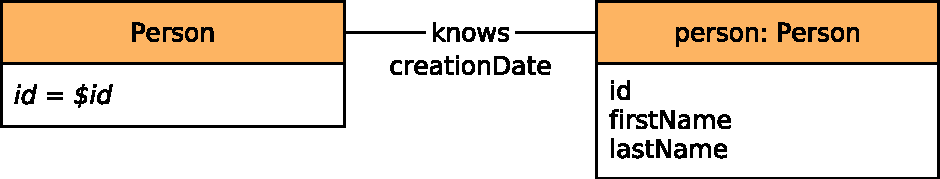
\includegraphics[scale=\patternscale,margin=0cm .2cm]{patterns/interactive-short-read-03}} \\ \hline
%
	desc. & Given a start Person, retrieve all of their friends, and the date at
which they became friends.
 \\ \hline
%
	
		params &
		\innerCardVSpace{\begin{tabularx}{\attributeCardWidth}{|>{\paramNumberCell}c|>{\varNameCell}M|>{\typeCell}m{\typeWidth}|Y|} \hline
		$\mathsf{1}$ & Person.id
 & ID
 &  \\ \hline
		\end{tabularx}}\innerCardVSpace \\ \hline
	
%
	
		result &
		\innerCardVSpace{\begin{tabularx}{\attributeCardWidth}{|>{\resultNumberCell}c|>{\varNameCell}M|>{\typeCell}m{\typeWidth}|>{\resultOriginCell}c|Y|} \hline
		$\mathsf{1}$ & Person.id & ID & R &
				 \\ \hline
		$\mathsf{2}$ & Person.firstName & String & R &
				 \\ \hline
		$\mathsf{3}$ & Person.lastName & String & R &
				 \\ \hline
		$\mathsf{4}$ & Knows.creationDate & DateTime & R &
				 \\ \hline
		\end{tabularx}}\innerCardVSpace \\ \hline
	
%
	
		sort		&
		\innerCardVSpace{\begin{tabularx}{\attributeCardWidth}{|>{\sortNumberCell}c|>{\varNameCell}M|>{\directionCell}c|Y|} \hline
		$\mathsf{1}$ & Knows.creationDate
 & $\desc
$ &  \\ \hline
		$\mathsf{2}$ & Person.id
 & $\asc
$ &  \\ \hline
		\end{tabularx}}\innerCardVSpace \\ \hline
	%
	%
	%
	%
\end{tabularx}
\queryCardVSpace

% change \emph back to the old one
\renewcommand{\emph}[1]{\oldemph{#1}}
\renewcommand*{\arraystretch}{1.1}

\subsection*{Interactive / short / 4}
\label{section:interactive-short-read-04}

% change \emph{} to use sans-serif font
\let\oldemph\emph
\renewcommand{\emph}[1]{{\footnotesize \sf #1}}



\noindent\begin{tabularx}{\queryCardWidth}{|>{\queryPropertyCell}p{\queryPropertyCellWidth}|X|}
	\hline
	query & Interactive / short / 4 \\ \hline
%
	title & Message Content \\ \hline
%
	pattern & \hfill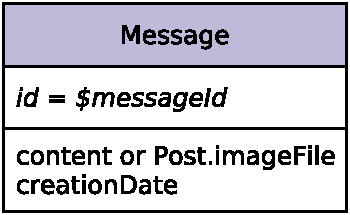
\includegraphics[scale=\patternscale,margin=0cm .2cm]{patterns/interactive-short-read-04}\hfill\vadjust{} \\ \hline
%
	desc. & Given a Message, retrieve its content and creation date.
 \\ \hline
%
	
		params &
		\innerCardVSpace{\begin{tabularx}{\attributeCardWidth}{|>{\paramNumberCell}c|>{\varNameCell}M|>{\typeCell}m{\typeWidth}|Y|} \hline
		$\mathsf{1}$ & Message.id
 & ID
 &  \\ \hline
		\end{tabularx}}\innerCardVSpace \\ \hline
	
%
	
		result &
		\innerCardVSpace{\begin{tabularx}{\attributeCardWidth}{|>{\resultNumberCell}c|>{\varNameCell}M|>{\typeCell}m{\typeWidth}|>{\resultOriginCell}c|Y|} \hline
		$\mathsf{1}$ & Message.creationDate & ID & R &
				 \\ \hline
		$\mathsf{2}$ & Message.content or Post.imageFile & String & R &
				 \\ \hline
		\end{tabularx}}\innerCardVSpace \\ \hline
	
%
	%
	%
	%
	%
\end{tabularx}
\queryCardVSpace

% change \emph back to the old one
\renewcommand{\emph}[1]{\oldemph{#1}}
\renewcommand*{\arraystretch}{1.1}

\noindent\begin{tabularx}{17cm}{|>{\small \sf}c|X|}
	\hline
	query    & Interactive / short / 5 \\ \hline
%
	title       & Message Creator \\ \hline
%
    pattern     & \hfill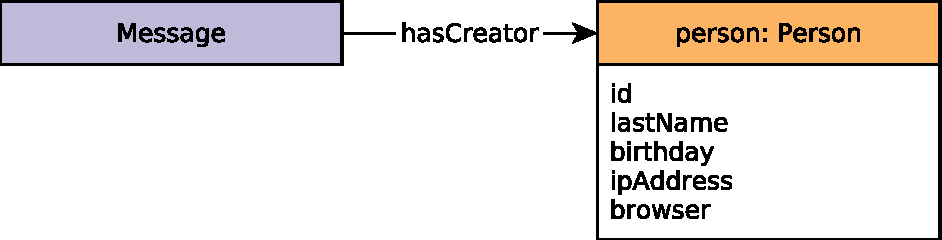
\includegraphics[scale=\patternscale,margin=0cm .2cm]{patterns/interactive-short-read-05}\hfill\vadjust{} \\ \hline
%
	desc. & Given a Message, retrieve its author.
 \\ \hline
%
	
%
	params.  &
	\vspace{1.1ex}{\begin{tabularx}{14.66cm}{|c|M|m{2cm}|Y|} \hline
	\cellcolor{parameter} \color{white} $\mathsf{1}$ & \varname{Message.id} & \cellcolor{gray!20} \vartype{ID} &  \\ \hline
	\end{tabularx}}\vspace{1.1ex} \\ \hline
%
	
	result      &
	\vspace{1.1ex}{\begin{tabularx}{14.66cm}{|c|M|m{2cm}|c|Y|} \hline
	\cellcolor{result} \color{white} $\mathsf{1}$ & \varname{Message-hasCreator->Person.id} & \cellcolor{gray!20} \vartype{ID} &
	    \texttt{R} &
	     \\ \hline
	\cellcolor{result} \color{white} $\mathsf{2}$ & \varname{Message-hasCreator->Person.firstName} & \cellcolor{gray!20} \vartype{String} &
	    \texttt{R} &
	     \\ \hline
	\cellcolor{result} \color{white} $\mathsf{3}$ & \varname{Message-hasCreator->Person.lastName} & \cellcolor{gray!20} \vartype{String} &
	    \texttt{R} &
	     \\ \hline
	\end{tabularx}}\vspace{1.1ex} \\ \hline
	
%
	%
	%
	%
    %
\end{tabularx}
\vspace{2ex}
\renewcommand*{\arraystretch}{1.1}

\subsection*{Interactive / short / 6}
\label{sec:interactive-short-read-06}

\noindent\begin{tabularx}{\queryCardWidth}{|>{\queryPropertyCell}c|X|}
	\hline
	query & Interactive / short / 6 \\ \hline
%
	title & Message Forum \\ \hline
%
    pattern & \hfill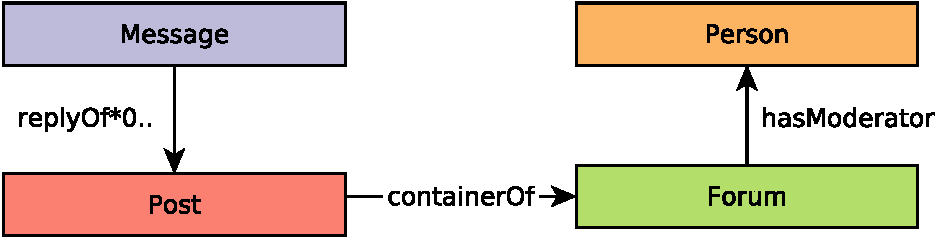
\includegraphics[scale=\patternscale,margin=0cm .2cm]{patterns/interactive-short-read-06}\hfill\vadjust{} \\ \hline
%
	desc. & Given a Message, retrieve the Forum that contains it and the Person that
moderates that forum. Since comments are not directly contained in
forums, for comments, return the forum containing the original post in
the thread which the comment is replying to.
 \\ \hline
%
	
%
    
        params &
        \innerCardVSpace{\begin{tabularx}{\attributeCardWidth}{|>{\paramNumberCell}c|>{\varNameCell}M|>{\typeCell}m{\typeWidth}|Y|} \hline
        \cellcolor{parameter} \color{white} \footnotesize $\mathsf{1}$ &Message.id& ID &  \\ \hline
        \end{tabularx}}\innerCardVSpace \\ \hline
	
%
	
        result &
        \innerCardVSpace{\begin{tabularx}{\attributeCardWidth}{|>{\resultNumberCell}c|>{\varNameCell}M|>{\typeCell}m{\typeWidth}|>{\resultOriginCell}c|Y|} \hline
        $\mathsf{1}$ & Message<-containerOf-Forum.id & ID &R&
                 \\ \hline
        $\mathsf{2}$ & Message<-containerOf-Forum.title & String &R&
                 \\ \hline
        $\mathsf{3}$ & Message<-containerOf-Forum-hasModerator->Person.id & ID &R&
                 \\ \hline
        $\mathsf{4}$ & Message<-containerOf-Forum-hasModerator->Person.firstName & String &R&
                 \\ \hline
        $\mathsf{5}$ & Message<-containerOf-Forum-hasModerator->Person.lastName & String &R&
                 \\ \hline
        \end{tabularx}}\innerCardVSpace \\ \hline
	
%
	%
	%
	%
    %
\end{tabularx}
\queryCardVSpace
\renewcommand*{\arraystretch}{1.1}

\subsection*{Interactive / short / 7}
\label{section:interactive-short-read-07}

% change \emph{} to use sans-serif font
\let\oldemph\emph
\renewcommand{\emph}[1]{{\footnotesize \sf #1}}



\noindent\begin{tabularx}{\queryCardWidth}{|>{\queryPropertyCell}p{\queryPropertyCellWidth}|X|}
	\hline
	query & Interactive / short / 7 \\ \hline
%
	title & Message Replies
 \\ \hline
%
	pattern & \hfill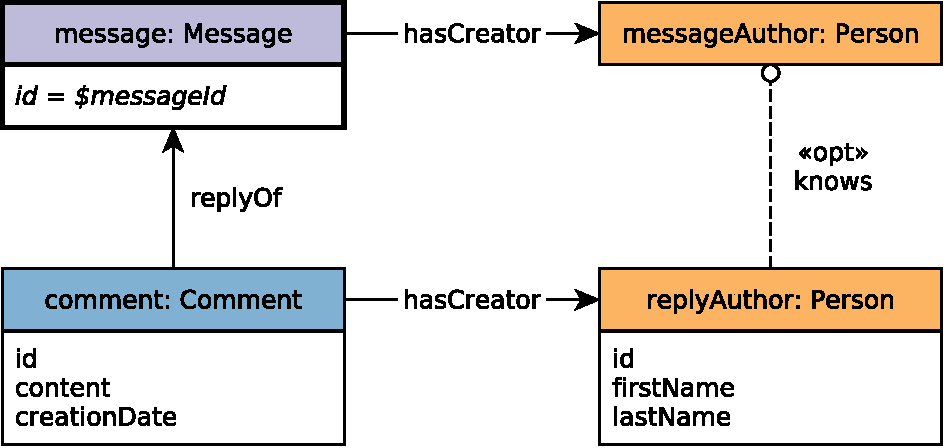
\includegraphics[scale=\patternscale,margin=0cm .2cm]{patterns/interactive-short-read-07}\hfill\vadjust{} \\ \hline
%
	desc. & Given a Message, retrieve the (1-hop) Comments that reply to it.

In addition, return a boolean flag \texttt{knows} indicating if the
author of the reply knows the author of the original message. If author
is same as original author, return false for \texttt{knows} flag.
 \\ \hline
%
	
		params &
		\innerCardVSpace{\begin{tabularx}{\attributeCardWidth}{|>{\paramNumberCell}c|>{\varNameCell}M|>{\typeCell}m{\typeWidth}|Y|} \hline
		$\mathsf{1}$ & Message.id
 & ID
 &  \\ \hline
		\end{tabularx}}\innerCardVSpace \\ \hline
	
%
	
		result &
		\innerCardVSpace{\begin{tabularx}{\attributeCardWidth}{|>{\resultNumberCell}c|>{\varNameCell}M|>{\typeCell}m{\typeWidth}|>{\resultOriginCell}c|Y|} \hline
		$\mathsf{1}$ & Message\textless{}-replyOf-Comment.id & ID & R &
				 \\ \hline
		$\mathsf{2}$ & Message\textless{}-replyOf-Comment.content & String & R &
				 \\ \hline
		$\mathsf{3}$ & Message\textless{}-replyOf-Comment.creationDate & DateTime & R &
				 \\ \hline
		$\mathsf{4}$ & Comment-hasCreator-\textgreater{}Person.id & ID & R &
				 \\ \hline
		$\mathsf{5}$ & Comment-hasCreator-\textgreater{}Person.firstName & String & R &
				 \\ \hline
		$\mathsf{6}$ & Comment-hasCreator-\textgreater{}Person.lastName & String & R &
				 \\ \hline
		$\mathsf{7}$ & knows & Boolean & C &
				Original message author knows reply author
 \\ \hline
		\end{tabularx}}\innerCardVSpace \\ \hline
	
%
	
		sort		&
		\innerCardVSpace{\begin{tabularx}{\attributeCardWidth}{|>{\sortNumberCell}c|>{\varNameCell}M|>{\directionCell}c|Y|} \hline
		$\mathsf{1}$ & Message\textless{}-replyOf-Comment.creationDate
 & $\desc
$ &  \\ \hline
		$\mathsf{2}$ & Message-hasCreator-\textgreater{}Person.id
 & $\asc
$ &  \\ \hline
		\end{tabularx}}\innerCardVSpace \\ \hline
	%
	%
	%
	%
\end{tabularx}
\queryCardVSpace

% change \emph back to the old one
\renewcommand{\emph}[1]{\oldemph{#1}}

%%%%%%%%%%%%%%%%%%%%%%%%%%%%%%%%%%%%%%%%%%%%%%%%%%%%%%%%%%%%%%%%%%%%%%%%%%%%%%
%%%%%%%%%%%%%%%%%%%%%%%%%%%%%%%%%%%%%%%%%%%%%%%%%%%%%%%%%%%%%%%%%%%%%%%%%%%%%%
%%%%%%%%%%%%%%%%%%%%%%%%%%%%%%%%%%%%%%%%%%%%%%%%%%%%%%%%%%%%%%%%%%%%%%%%%%%%%%

\section{Inserts}
\label{sec:inserts}

Each insert query inserts either (1) a single node of a certain type, along with its edges to other existing nodes or (2) a single edge of a certain type between two existing nodes.

\input{query-cards/interactive-insert-01}
\input{query-cards/interactive-insert-02}
\input{query-cards/interactive-insert-03}
\input{query-cards/interactive-insert-04}
\input{query-cards/interactive-insert-05}
\input{query-cards/interactive-insert-06}
\input{query-cards/interactive-insert-07}
\input{query-cards/interactive-insert-08}

\section{Deletes}
\label{sec:deletes}

Each delete query removes either (1) a single edge between two existing vertices or (2) a vertex, all incident edges and transitive vertices (where appropriate).

\renewcommand*{\arraystretch}{1.1}

\subsection{Interactive / delete / 1}
\label{sec:interactive-delete-01}

% change \emph{} to use sans-serif font
\let\oldemph\emph
\renewcommand{\emph}[1]{{\footnotesize \sf #1}}

\renewcommand{\currentQueryCard}{1}
\marginpar{
	\raggedleft
	\vspace{0.22ex}

	\queryRefCard{interactive-delete-01}{ID}{1}\\
	\queryRefCard{interactive-delete-02}{ID}{2}\\ 
	\queryRefCard{interactive-delete-03}{ID}{3}\\
	\queryRefCard{interactive-delete-04}{ID}{4}\\
	\queryRefCard{interactive-delete-05}{ID}{5}\\
	\queryRefCard{interactive-delete-06}{ID}{6}\\
	\queryRefCard{interactive-delete-07}{ID}{7}\\
	\queryRefCard{interactive-delete-08}{ID}{8}\\
}


\noindent\begin{tabularx}{\queryCardWidth}{|>{\queryPropertyCell}p{\queryPropertyCellWidth}|X|}
\hline
query & Interactive / delete / 1 \\ \hline
%
title & Remove person \\ \hline
%
% pattern & \centering 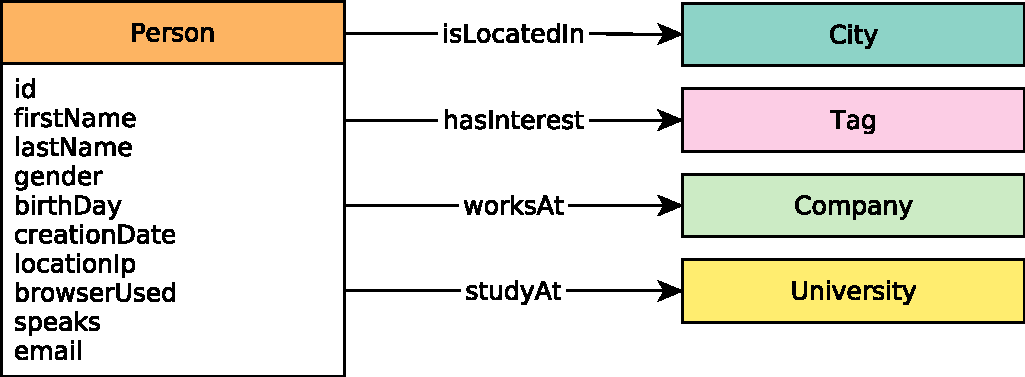
\includegraphics[scale=\patternscale,margin=0cm .2cm]{patterns/interactive-update-01} \tabularnewline \hline
%
desc. & Remove a \emph{Person} \textbf{node} and it's incident \textbf{edges} (\emph{isLocatedIn}, \emph{studyAt}, \emph{workAt}, \emph{hasInterest}, \emph{likes}, \emph{knows}, \emph{hasMember}, \emph{hasModerator}, \emph{hasCreator}). The removal of a \emph{Person} removes all \emph{Forum} they are moderator of and all messages they have posted in other forums. 
\\ \hline
%
params & \innerCardVSpace{\begin{tabularx}{\attributeCardWidth}{|>{\paramNumberCell}c|>{\varNameCell}M|>{\typeCell}m{\typeWidth}|Y|} \hline $\mathsf{1}$ & Person.id & ID & \texttt{forumId} \\ \hline
\end{tabularx}}\innerCardVSpace \\ \hline	
%	
comments &
\begin{itemize}
  \item Removal of a person can (1) remove all associated posts/comments/forum nodes or (2) just the person node. GDPR is a valid argument for (1). Approach (2) could lead to problems with read queries, driver gathering parameters for short reads and inadvertently impose implementation decisions for implementors. 
\item Removal of a person removes forums of type ``personal walls'' and ``image albums'' not ``groups'', which can continue if even the founder has left the network. The hasModerator edge must transition to an existing person node in the network, two approaches to assigning a new moderator were discussed: (1) choose member at random from the set of existing group members or (2) the member with the oldest group join date becomes the moderator.   
\item Removal of a person removes all posts/comments they are creator of this could result in the removal of a comment in the middle of a thread. 
\end{itemize}
 \\ \hline
%
% 
%
%
\end{tabularx}
\queryCardVSpace

% change \emph back to the old one
\let\emph\oldemph



\input{query-cards/interactive-delete-02}
\renewcommand*{\arraystretch}{1.1}

\subsection{Interactive / delete / 3}
\label{sec:interactive-delete-03}

% change \emph{} to use sans-serif font
\let\oldemph\emph
\renewcommand{\emph}[1]{{\footnotesize \sf #1}}

\renewcommand{\currentQueryCard}{3}
\marginpar{
  \raggedleft
  \vspace{0.22ex}

  \queryRefCard{interactive-delete-01}{ID}{1}\\
  \queryRefCard{interactive-delete-02}{ID}{2}\\ 
  \queryRefCard{interactive-delete-03}{ID}{3}\\
  \queryRefCard{interactive-delete-04}{ID}{4}\\
  \queryRefCard{interactive-delete-05}{ID}{5}\\
  \queryRefCard{interactive-delete-06}{ID}{6}\\
  \queryRefCard{interactive-delete-07}{ID}{7}\\
  \queryRefCard{interactive-delete-08}{ID}{8}\\
}


\noindent\begin{tabularx}{\queryCardWidth}{|>{\queryPropertyCell}p{\queryPropertyCellWidth}|X|}
  \hline
  query & Interactive / delete / 3 \\ \hline
  % 
  title & Remove comment like \\ \hline
  % 
  % pattern & \centering 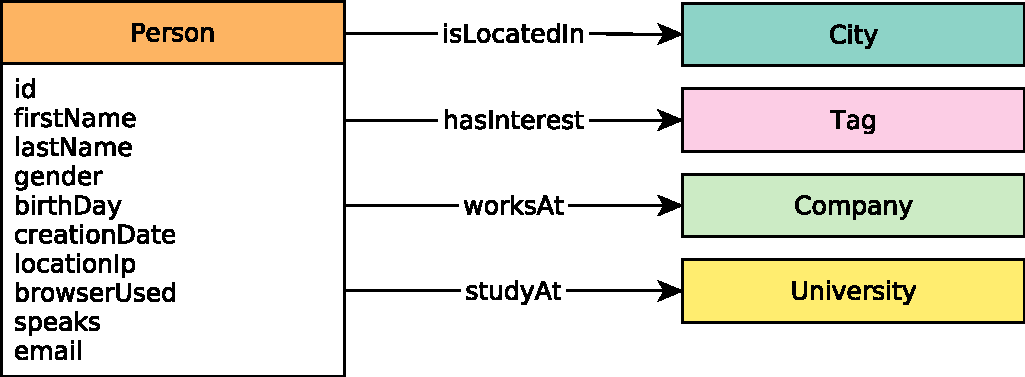
\includegraphics[scale=\patternscale,margin=0cm .2cm]{patterns/interactive-update-01} \tabularnewline \hline
  % 
  desc. & Given a \emph{Person} \textbf{node} and a \emph{Comment} \textbf{node}, remove a \emph{likes} edge between them.
  \\ \hline
  % 
  params &
  \innerCardVSpace{\begin{tabularx}{\attributeCardWidth}{|>{\paramNumberCell}c|>{\varNameCell}M|>{\typeCell}m{\typeWidth}|Y|} \hline
      $\mathsf{1}$ & Person.id
      & ID
      & \texttt{personId}
      \\ \hline
      $\mathsf{2}$ & Comment.id
      & ID
      & \texttt{commentId}
      \\ \hline
    \end{tabularx}}\innerCardVSpace \\ \hline
  % 
  comments &
  \begin{itemize}
  \item Removal a likes edge is a rare event e.g. people accidently liking a comment, this can be reflected by the relative frequency of the operation.   
  \end{itemize} 
  \\ \hline
  % 
  % 
  % 
  % 
  % 
\end{tabularx}
\queryCardVSpace

% change \emph back to the old one
\let\emph\oldemph

\renewcommand*{\arraystretch}{1.1}

\subsection{Interactive / delete / 4}
\label{sec:interactive-delete-04}

% change \emph{} to use sans-serif font
\let\oldemph\emph
\renewcommand{\emph}[1]{{\footnotesize \sf #1}}

\renewcommand{\currentQueryCard}{4}
\marginpar{
	\raggedleft
	\vspace{0.22ex}

	\queryRefCard{interactive-delete-01}{ID}{1}\\
	\queryRefCard{interactive-delete-02}{ID}{2}\\ 
	\queryRefCard{interactive-delete-03}{ID}{3}\\
	\queryRefCard{interactive-delete-04}{ID}{4}\\
	\queryRefCard{interactive-delete-05}{ID}{5}\\
	\queryRefCard{interactive-delete-06}{ID}{6}\\
	\queryRefCard{interactive-delete-07}{ID}{7}\\
	\queryRefCard{interactive-delete-08}{ID}{8}\\
}


\noindent\begin{tabularx}{\queryCardWidth}{|>{\queryPropertyCell}p{\queryPropertyCellWidth}|X|}
	\hline
	query & Interactive / delete / 4 \\ \hline
%
	title & Remove forum membership \\ \hline
%
	% pattern & \centering 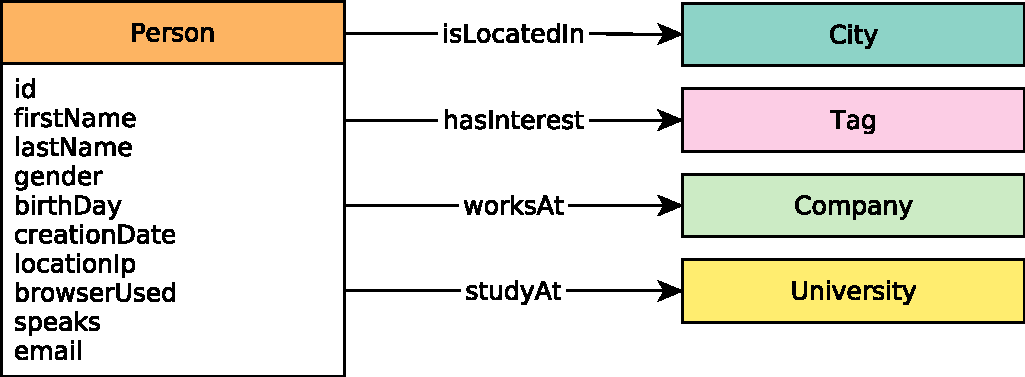
\includegraphics[scale=\patternscale,margin=0cm .2cm]{patterns/interactive-update-01} \tabularnewline \hline
%
	desc. & Given a \emph{Forum} \textbf{node} and a \emph{Person} \textbf{node}, remove a \emph{hasMember} edge between them. 
 \\ \hline
%
	
		params &
		\innerCardVSpace{\begin{tabularx}{\attributeCardWidth}{|>{\paramNumberCell}c|>{\varNameCell}M|>{\typeCell}m{\typeWidth}|Y|} \hline
		$\mathsf{1}$ & Forum.id
 & ID
 & \texttt{forumId}
 \\ \hline
		$\mathsf{2}$ & Person.id
 & ID
 & \texttt{personId}
 \\ \hline
		\end{tabularx}}\innerCardVSpace \\ \hline
	
%
	
%
	%
	%
	%
	%
\end{tabularx}
\queryCardVSpace

% change \emph back to the old one
\let\emph\oldemph
\input{query-cards/interactive-delete-05}
\renewcommand*{\arraystretch}{1.1}

\subsection{Interactive / delete / 6}
\label{sec:interactive-delete-06}

% change \emph{} to use sans-serif font
\let\oldemph\emph
\renewcommand{\emph}[1]{{\footnotesize \sf #1}}

\renewcommand{\currentQueryCard}{6}
\marginpar{
	\raggedleft
	\vspace{0.22ex}

	\queryRefCard{interactive-delete-01}{ID}{1}\\
	\queryRefCard{interactive-delete-02}{ID}{2}\\ 
	\queryRefCard{interactive-delete-03}{ID}{3}\\
	\queryRefCard{interactive-delete-04}{ID}{4}\\
	\queryRefCard{interactive-delete-05}{ID}{5}\\
	\queryRefCard{interactive-delete-06}{ID}{6}\\
	\queryRefCard{interactive-delete-07}{ID}{7}\\
	\queryRefCard{interactive-delete-08}{ID}{8}\\
}


\noindent\begin{tabularx}{\queryCardWidth}{|>{\queryPropertyCell}p{\queryPropertyCellWidth}|X|}
	\hline
	query & Interactive / delete / 6 \\ \hline
%
	title & Remove post \\ \hline
%
	% pattern & \centering 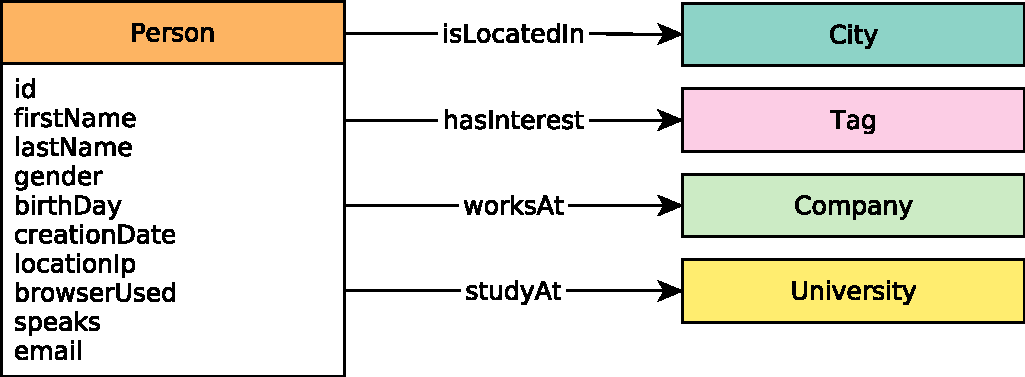
\includegraphics[scale=\patternscale,margin=0cm .2cm]{patterns/interactive-update-01} \tabularnewline \hline
%
	desc. & Remove a \emph{Post} \textbf{node} and it's incident \textbf{edges} (\emph{isLocatedIn}, \emph{likes}, \emph{hasCreator}, \emph{hasTag}, \emph{containerOf}). Remove all replies (connected by \emph{replyOf}) to the \emph{Post} and their incident \textbf{edges}. In addition, remove all transitive replies to the \emph{Post} and their incident \textbf{edges}.
 \\ \hline
%
	
		params &
		\innerCardVSpace{\begin{tabularx}{\attributeCardWidth}{|>{\paramNumberCell}c|>{\varNameCell}M|>{\typeCell}m{\typeWidth}|Y|} \hline
		$\mathsf{1}$ & Post.id
 & ID
 & \texttt{postId}
 \\ \hline
		\end{tabularx}}\innerCardVSpace \\ \hline
	
%
	
%
	%
	%
	%
	%
\end{tabularx}
\queryCardVSpace

% change \emph back to the old one
\let\emph\oldemph
\renewcommand*{\arraystretch}{1.1}

\subsection{Interactive / delete / 7}
\label{sec:interactive-delete-07}

% change \emph{} to use sans-serif font
\let\oldemph\emph
\renewcommand{\emph}[1]{{\footnotesize \sf #1}}

\renewcommand{\currentQueryCard}{7}
\marginpar{
	\raggedleft
	\vspace{0.22ex}

	\queryRefCard{interactive-delete-01}{ID}{1}\\
	\queryRefCard{interactive-delete-02}{ID}{2}\\ 
	\queryRefCard{interactive-delete-03}{ID}{3}\\
	\queryRefCard{interactive-delete-04}{ID}{4}\\
	\queryRefCard{interactive-delete-05}{ID}{5}\\
	\queryRefCard{interactive-delete-06}{ID}{6}\\
	\queryRefCard{interactive-delete-07}{ID}{7}\\
	\queryRefCard{interactive-delete-08}{ID}{8}\\
}


\noindent\begin{tabularx}{\queryCardWidth}{|>{\queryPropertyCell}p{\queryPropertyCellWidth}|X|}
	\hline
	query & Interactive / delete / 7 \\ \hline
%
	title & Remove comment \\ \hline
%
	% pattern & \centering 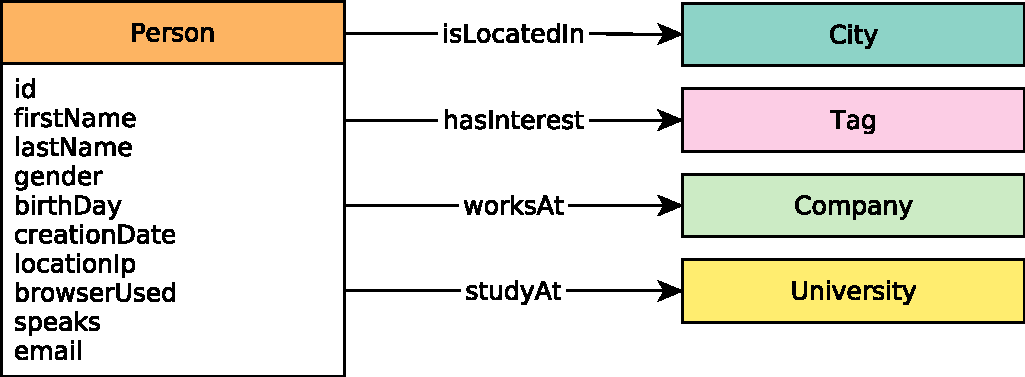
\includegraphics[scale=\patternscale,margin=0cm .2cm]{patterns/interactive-update-01} \tabularnewline \hline
%
	desc. & Remove a \emph{Comment} \textbf{node} and it's incident \textbf{edges} (\emph{isLocatedIn}, \emph{likes}, \emph{hasCreator}, \emph{hasTag}). In addition, remove all replies to the \emph{Comment} connected by \emph{replyOf} and their incident \textbf{edges}. 
 \\ \hline
%
	
		params &
		\innerCardVSpace{\begin{tabularx}{\attributeCardWidth}{|>{\paramNumberCell}c|>{\varNameCell}M|>{\typeCell}m{\typeWidth}|Y|} \hline
		$\mathsf{1}$ & Comment.id
 & ID
 & \texttt{CommentId}
 \\ \hline
		\end{tabularx}}\innerCardVSpace \\ \hline
	
%
	
%
	%
	%
	%
	%
\end{tabularx}
\queryCardVSpace

% change \emph back to the old one
\let\emph\oldemph

\renewcommand*{\arraystretch}{1.1}

\subsection{Interactive / delete / 8}
\label{sec:interactive-delete-08}

% change \emph{} to use sans-serif font
\let\oldemph\emph
\renewcommand{\emph}[1]{{\footnotesize \sf #1}}

\renewcommand{\currentQueryCard}{8}
\marginpar{
	\raggedleft
	\vspace{0.22ex}

	\queryRefCard{interactive-delete-01}{ID}{1}\\
	\queryRefCard{interactive-delete-02}{ID}{2}\\ 
	\queryRefCard{interactive-delete-03}{ID}{3}\\
	\queryRefCard{interactive-delete-04}{ID}{4}\\
	\queryRefCard{interactive-delete-05}{ID}{5}\\
	\queryRefCard{interactive-delete-06}{ID}{6}\\
	\queryRefCard{interactive-delete-07}{ID}{7}\\
	\queryRefCard{interactive-delete-08}{ID}{8}\\
}


\noindent\begin{tabularx}{\queryCardWidth}{|>{\queryPropertyCell}p{\queryPropertyCellWidth}|X|}
	\hline
	query & Interactive / delete / 8 \\ \hline
%
	title & Remove friendship \\ \hline
%
	% pattern & \centering 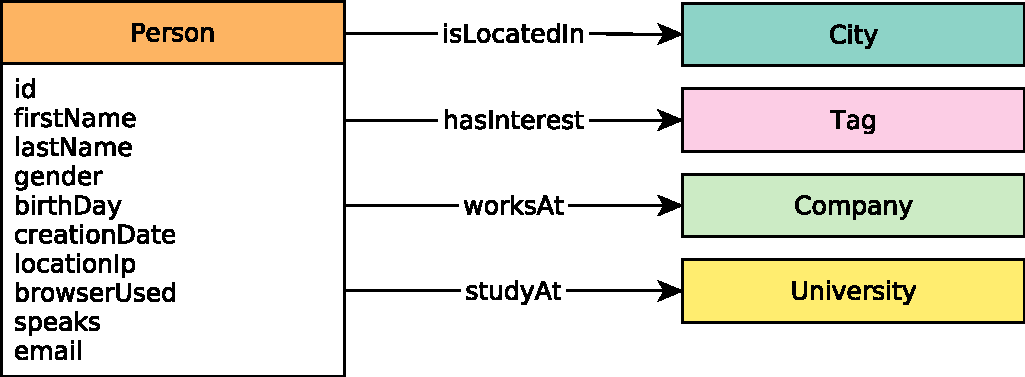
\includegraphics[scale=\patternscale,margin=0cm .2cm]{patterns/interactive-update-01} \tabularnewline \hline
%
	desc. & Given two \emph{Person} \textbf{nodes}, remove a \emph{knows} edge between them. 
 \\ \hline
%
	
		params &
		\innerCardVSpace{\begin{tabularx}{\attributeCardWidth}{|>{\paramNumberCell}c|>{\varNameCell}M|>{\typeCell}m{\typeWidth}|Y|} \hline
		$\mathsf{1}$ & Person.id
 & ID
 & \texttt{person1Id}
 \\ \hline
		$\mathsf{2}$ & Person.id
 & ID
 & \texttt{person2Id}
 \\ \hline
		\end{tabularx}}\innerCardVSpace \\ \hline
	
%
	
%
	%
	%
	%
	%
\end{tabularx}
\queryCardVSpace

% change \emph back to the old one
\let\emph\oldemph


% reset counter to make sure the last query card isn't stuck in highlighted mode
\renewcommand{\currentQueryCard}{0}
